\documentclass[11pt]{article}

\usepackage{amsmath}
\usepackage{amsfonts}
\usepackage{amssymb}
\usepackage{graphicx}
\usepackage[center]{caption}
\usepackage{mathtools}
\usepackage{lipsum}
\usepackage{stackengine}
\usepackage{fancyhdr}
\usepackage{caption}
\usepackage{tikz}
\usetikzlibrary{shapes.geometric, arrows}
\usepackage{float}
\usepackage[a4paper,left=1in,right=1in,top=1in,bottom=1in,footskip=.25in]{geometry}
\usepackage{etoolbox}
\usepackage[nottoc]{tocbibind}
\usepackage{tabu}
\usepackage{enumitem,kantlipsum}
\usepackage{verbatim}
\usepackage{hyperref}
\begin{document}
\begin{titlepage}
	\centering
	
	\begin{figure}
		\begin{center}
			
\includegraphics[scale=.2]{tubaf.pdf}  
		\end{center}
		
	\end{figure}
	

	
	
	
	%\includegraphics[width=0.15\textwidth]{download}\par\vspace{1cm}
	{\scshape\LARGE Technische Universit\"at Bergakademie Freiberg \par}
	\vspace{1cm}
	{\scshape\Large PERSONAL PROGRAMMING PROJECT\par}
	\vspace{1.5cm}
	{\huge\bfseries Implementation of Iso-geometric Analysis (IGA) for
		Piezoelectric Material \par}
	\vspace{2cm}
	{\scshape\Large Vikas Diddige\par}
	{\scshape\Large 64041\par}
	\vfill
	{\normalsize\ Supervised by\par}
	
	Dr.~ \textsc{Sergii Kozinov}
	
	\vfill
	
	% Bottom of the page
	{\large \today\par}
\end{titlepage}

\clearpage

\newpage
\clearpage
\tableofcontents
\clearpage

\vspace*{1cm}

\section{Introduction}
Among all the numerical methods, Finite Element Methods (FEM) are more popularly used to find approximate solutions of partial differential equations. FEM approximates the Computer Aided Drawing (CAD) geometry by discretizing it into smaller geometries called elements. Such geometrical approximations may create numerical errors and seriously affect the accuracy of the solution. Isogeometric analysis (IGA), on the other hand, is a technique to generate geometry using CAD concept of Non-Uniform Rational B-Splines (NURBS) and analyze using its basis functions \cite{agrawal2019iga}. With the use of NURBS basis functions instead of Lagrangian basis functions, the geometry is captured exactly for the analysis and rules out the possibility of the geometrical errors. Moreover, the time from design to analysis phase is greatly reduced, saving the cost and time for the industry. The IGA technique is firstly pioneered by Tom Hughes and his group at The University of Texas at Austin.\\
\par
In the present programming project, python code is developed, which can generate any 2D NURBS surface, given the physical and parametric details of the geometry. Few commercial software (for example, Rhino) can be used to get the parametric details of the surface. Later the code is extended to analyze the linear elastic mechanical loading case as a displacement driven algorithm. Further, the electro-mechanical coupling is added. The written code gives accurate results for a 2nd order NURBS basis functions. For higher-order basis functions, a particular treatment is required for defining boundary conditions like least square minimization technique. The results have been verified using Abaqus results. Comparing the IGA program generated results with Abaqus elements output is justified because IGA aims at reducing the approximation from traditional FEM procedures.    

\subsection{Advantages of IGA over FEA}
\begin{description}[leftmargin=*]
	\item[$\bullet$]   The exact representation of the geometry for analysis rules
	out the possibility of geometrical approximations.
	\item[$\bullet$]   A huge amount of time and effort involved in finite element modelling
	can be avoided.
\end{description}

\newpage

\section{B-Splines } \label{B_Spline}
In this section, a brief description of B-Splines is discussed since NURBS is an extended version of B-Splines. A B-Spline basis function is defined by its order and knot vectors. A B-spline basis function, along with control points, defines a B-Spline curve. A surface or volume can be generated using a curve by tensor product between its basis functions, which will be discussed in detail in the future sections.
\begin{figure}[H]
	\begin{center}
		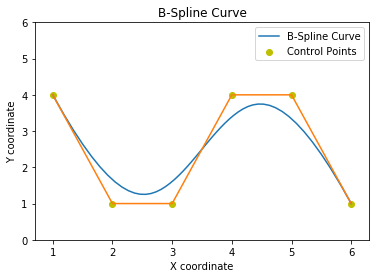
\includegraphics[scale=0.8]{B_Spline.png} 
		\caption{\\A B-Spline curve with six control points}\label{B_Spline}
	\end{center}	
\end{figure}
\subsection{Order }
For a point on a B-Spline curve, the order of the basis function speaks about the number of nearby control points that influence the given point. The degree $p$ of the basis function is one less than the order of the curve. The following figure shows a B-Spline curve with the same number and position of control points but with different orders.
\begin{figure}[H]
	\begin{center}
		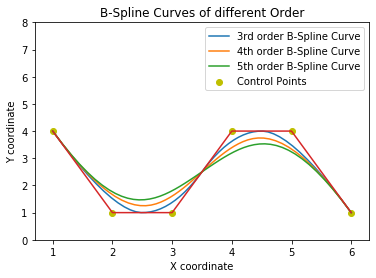
\includegraphics[scale=0.8]{DegreeBspline.png} 
		\caption{\\B-Spline curves with same control points but different order}\label{DegreeBspline}
	\end{center}	
\end{figure}

\subsection{Knot vector } \label{KnotVectorSection}
A knot vector is an array with an ascending order of parameter values written as $\Xi = \{ \xi_0,\xi_1,\xi_2.....,\xi_{n+p}\}$ ($\xi_i$ is called $ith$ knot and $\{\xi_i,\xi_{i+1}\}$ is called $ith$ Knot span), with $n+1$ basis functions which will be discussed in later sections. The number of knots in a knot vector is equal to the summation of the degree of the curve and total number of control points defining the curve. B-Spline curves are defined in parametric space which is divided by knot spans. Knot vector should be an ascending order of knots. For example $\{0,0,1,1,2,3,3\}$ is valid but not $\{0,0,1,2,3,2,3\}$. There is no difference between $\Xi = \{0,0,0,1,2,3,4,4,4\}$ and $\Xi = \{0,0,0,1/4,2/4,3/4,1,1,1\}$ which can be seen from Fig.(\ref{SameKnotVector}) because the latter can be obtained by dividing the former by 4.
\begin{figure}[H]
	\begin{center}
		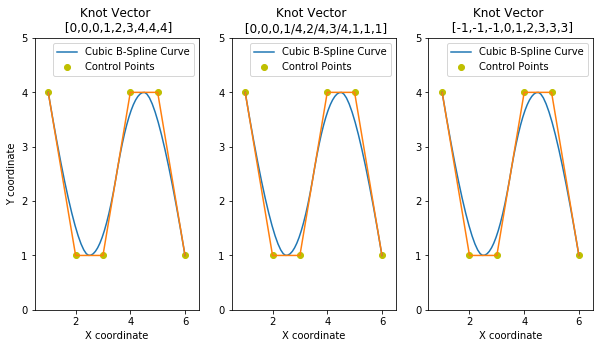
\includegraphics[scale=0.8]{SameKnotVector.png} 
		\caption{\\B-Spline curves showing same trend with different Knot Vectors}\label{SameKnotVector}
	\end{center}	
\end{figure}
The effect of the control points on a B-Spline curve is completely defined by knot vector parameter values as shown in Fig.(\ref{DifferentKnotVector}).
\begin{figure}[H]
	\begin{center}
		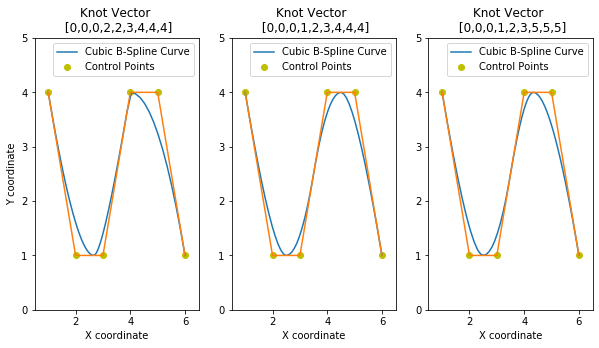
\includegraphics[scale=0.8]{DifferentKnotVector.png} 
		\caption{\\B-Spline curves with same control points but with different Knot vectors}\label{DifferentKnotVector}
	\end{center}	
\end{figure}

\subsection{Control points }
The co-ordinates and number of the control points determine the shape of the curve, and the shape can be varied by altering the knot values in the knot vector, as discussed in section (\ref{KnotVectorSection}). A span on the B-Spline curve is controlled by $p+1$ number of points. The total number of control points is given by $n_{cp}(\xi)$ = total number of knots in
$[\Xi] - (p+1)$. For a $pth$ degree curve, at least $p+1$ control points have to be defined. 


\subsection{B-Spline basis functions }

For a given Knot vector $\Xi$, the B-spline basis function for polynomial degree $\geq 1$ is defined by a recursive function \cite{piegl2012nurbs}

\begin{equation}
N_{i,p}(\xi) = \frac{\xi-\xi_{i}}{\xi_{i+p}-\xi_{i}} N_{i,p-1}(\xi) + 
\frac{\xi_{i+p+1}-\xi}{\xi_{i+p+1}-\xi_{i+1}} N_{i+1,p-1}(\xi)
\end{equation}

\noindent
with
\begin{equation}
N_{i,0}(\xi) = 
\begin{cases*}
1 \quad& if $  \xi_{i} \leq \xi<\xi_{i+1} $ \\
0 &  $ otherwise $ \\
\end{cases*}
\end{equation}

\subsubsection{Properties }
\begin{enumerate}
	\item $ N_{i,0}(\xi)$ is a step wise function with a value 1 over the half open interval $ \xi \in [\xi_{i}  \leq \xi<\xi_{i+1}) $ and zero on the rest. 
	\item Basis functions sum upto to unity $\sum_{i=0}^{n} N_{i,p}(\xi) =1$.
	\item Basis functions are non-negative $ N_{i,p}(\xi) \geq 0$ over the entire domain.
\end{enumerate}

\begin{figure}[H]
	\begin{center}
		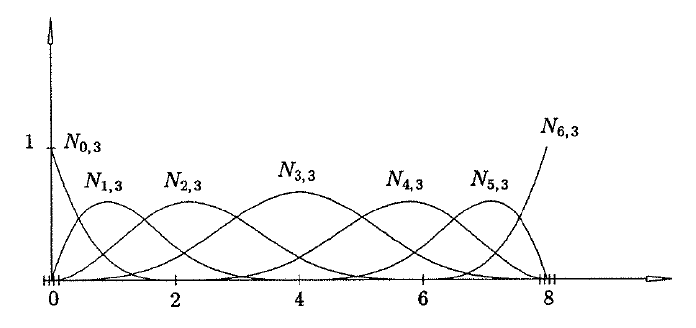
\includegraphics[scale=0.7]{BSplineBasisFunctions.png}
		\caption{\\Cubic B-Spline functions with a uniform knot vector \cite{piegl2012nurbs}   }\label{BSplineBasisFunctions}
	\end{center}	
\end{figure}
\noindent
The following python function outputs non zero basis functions in a given knot vector span
\begin{verbatim}
-----------------------------------------------------------------------------------
def BasisFuns(i,u,p,U):
#----------Inputs---------#
i - knot span
u - parametric coordinate
p - Degree of the curve
U - knot vector of the curve
#----------Outputs---------#
non zero basis functions for the given parametric coordinate
-----------------------------------------------------------------------------------
\end{verbatim}

\subsubsection{Derivatives }
The first derivative of a B-Spline basis function \cite{nguyen2012introduction} with its variable $\xi$ is
given by

\begin{equation}
\frac{d}{d\xi}N_{i,p}(\xi) = \frac{p}{\xi_{i+p}-\xi_{i}} N_{i,p-1}(\xi) -
\frac{p}{\xi_{i+p+1}-\xi_{i+1}} N_{i+1,p-1}(\xi)
\end{equation}

\noindent
Higher-order derivatives are not necessary for IGA formulation.\\
The following python function outputs derivatives of non zero basis functions in a given knot vector span.
\begin{verbatim}
-----------------------------------------------------------------------------------
def DersBasisFuns(i,u,p,m,U):
#----------Inputs---------#
i - knot span
u - parametric coordinate
p - Degree of the curve
U - knot vector of the curve
m - derivatives upto and including m(th) 
#----------Outputs---------#
The function returns non zero basis functions and their derivatives
upto and including mth derivative for the given parametric coordinate
-----------------------------------------------------------------------------------
\end{verbatim}

\subsection{B-Spline curves}

A $pth-degree$ B-Spline curve with a set of control points $P_i$ is given by \cite{piegl2012nurbs}
\begin{equation}
C(\xi) = \sum_{i=0}^{n} N_{i,p}(\xi) P_i \qquad \xi_0 \leq \xi \leq \xi_{n+p}
\end{equation}

\noindent
defined on the knot vector $\Xi = \{ \xi_0,\xi_1,\xi_2.....,\xi_{n+p}\}$

\subsection{B-Spline surfaces}
A B-Spline surface $S(\xi,\eta)$ is built by tensor product between B-Spline
curves along each parametric direction ($\xi,\eta$). It requires knot vectors
($\Xi = \{ \xi_0,\xi_1,\xi_2.....,\xi_{n+p}\}$,$H =
\{\eta_0,\eta_1,\eta_2.....,\eta_{m+q}\}$) along each parametric direction and
control net $P_{i,j}$
\begin{figure}[H]
	\begin{center}
		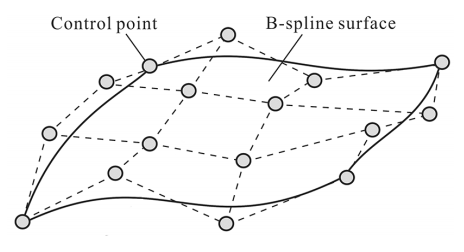
\includegraphics[scale=0.7]{B_Spline_Surface.png} 
		\caption{\\A B-Spline surface with control points net \cite{siggel2017tigl}}\label{B_Spline_Surface}
	\end{center}	
\end{figure}


\begin{equation} \label{BSplineSurface}
S(\xi,\eta) = \sum_{i=0}^{n}\sum_{j=0}^{m} N_{i,p}(\xi) N_{j,q}(\eta) P_{i,j}
\end{equation}

\noindent
where p,q are the degrees of the B-Spline basis functions along $\xi,\eta$ directions respectively, and n,m are the number of control points along $\xi,\eta$ directions respectively.
\noindent
Eq. (\ref{BSplineSurface}) can be compactly written as


\begin{equation} \label{BSplineSurface}
S(\xi,\eta) = \sum_{i=0}^{n}\sum_{j=0}^{m} N_{i,j}^{p,q}(\xi,\eta) P_{i,j}
\end{equation}

\subsubsection{Derivatives}

The partial derivatives of bivariate B-Spline basis functions w.r.t parametric coordinates are given as \cite{nguyen2012introduction}

\begin{equation} 
\frac{\partial N_{i,j}^{p,q}(\xi,\eta)}{\partial \xi} = \frac{d}{d\xi}
\bigg(N_{i,p}(\xi)\bigg)N_{j,q}(\eta) 
\qquad
\frac{\partial N_{i,j}^{p,q}(\xi,\eta)}{\partial \eta} = \frac{d}{d\eta}
\bigg(N_{j,q}(\eta)\bigg)N_{i,p}(\xi)
\end{equation}

\newpage
\section{Non Uniform Rational B-Splines } \label{NURBS}
NURBS are very often used in computer-aided design(CAD), manufacturing (CAM) and engineering (CAE) due to its flexibility to represent complex geometries. NURBS curves and surfaces are considered as the generalization of B-Spline and Bezier curves and surfaces. A NURBS basis function is defined by its order and knot vector.

\subsection{NURBS basis functions}
NURBS basis functions $R_{i,p}(\xi)$ are defined as \cite{piegl2012nurbs}
\begin{equation}\label{NURBSBasisFuncs}
R_{i,p}(\xi) = \frac{N_{i,p}(\xi)w_{i}}{\sum_{i=0}^{n}N_{i,p}(\xi)w_{i}}
\end{equation}

\noindent
where $N_{i,p}(\xi)$ is the $i$th B-Spline basis function with degree p and $w_{i}$ denotes weight of the $i$th control point ($P_i$). When $w_{i} = constant \quad \forall i$ the NURBS basis function reduces to B-Spline basis function. \\The usage of weights can be illustrated in Fig.(\ref{WeightsCircles}). The same circle can be drawn with different number of control points by altering their weights.
\begin{figure}[H]
	\begin{center}
		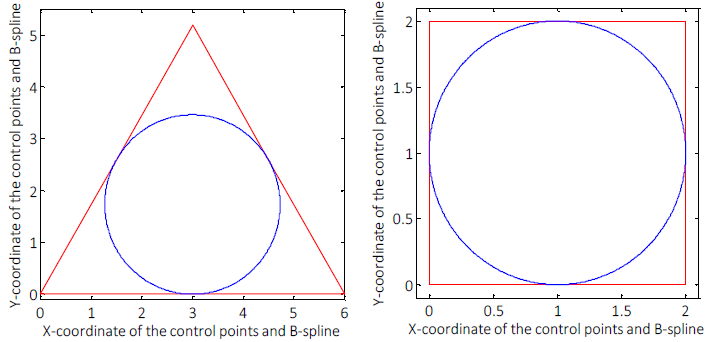
\includegraphics[scale=0.7]{WeightsCircles.png} 
		\caption{\\NURBS circle with different control points and weights \cite{shah2015stress}}\label{WeightsCircles}
	\end{center}	
\end{figure}

\subsubsection{Derivatives}
The first derivative of a NURBS basis function with its variable $\xi$ is given by \cite{nguyen2012introduction}

\begin{equation}
\frac{d }{d \xi} R_{i,p}(\xi) = \frac{N^{'}_{i,p}(\xi)  W(\xi) - N_{i,p}(\xi) 
	W^{'}(\xi)}{W^{2}(\xi)}w_{i}
\end{equation}
\noindent
where
$N^{'}_{i,p}(\xi) = \frac{d }{d \xi} N_{i,p}(\xi)$  \\
\\
\noindent
and $W^{'}(\xi) =  \sum_{i=0}^{n}N^{'}_{i,p}(\xi) w_i$


\subsection{NURBS Curves }
The $p^{th}$ degree NURBS curve is given by \cite{piegl2012nurbs}

\begin{equation}
C(\xi) =
\frac{\sum_{i=0}^{n}N_{i,p}(\xi)w_{i}P_{i}}{\sum_{i=0}^{n}N_{i,p}(\xi)w_{i}}
\qquad \xi_0 \leq \xi \leq \xi_{n+p}
\end{equation}
in short form
\begin{equation}
C(\xi) = \sum_{i=0}^{n}R_{i,p}(\xi)P_{i}
\end{equation}
\\
A NURBS curve with different weights on control points along with its basis function is shown in Fig. (\ref{NURBSCurveBasisFunctions})
\begin{figure}[H]
	\begin{center}
		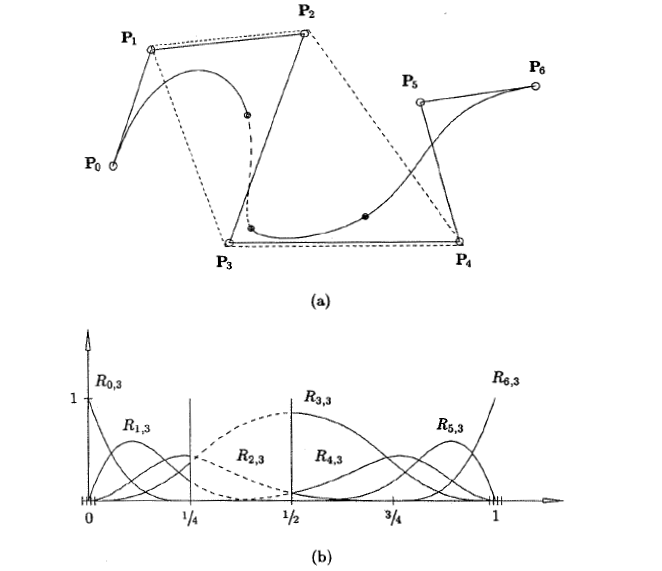
\includegraphics[scale=0.7]{NURBSCurveBasisFunctions.png} 
		\caption{\\$\Xi=\{0,0,0,0,1,2,3,4,4,4,4\}, w = \{1,1,1,3,1,1,1\}$\\(a) A third degree NURBS curve; (b) Associated NURBS basis functions \cite{piegl2012nurbs}}\label{NURBSCurveBasisFunctions}
	\end{center}	
\end{figure}
\subsubsection{Properties }
\begin{enumerate}
	\item NURBS basis functions sum upto to unity $\sum_{i=0}^{n} R_{i,p}(\xi) =1$
	\item NURBS basis functions are non-negative $ R_{i,p}(\xi) \geq 0$ over the entire
	domain
	\item $R_{0,p}(0)=R_{n,p}(1)=1$
	\item For $w_i=1$ for all $i$, NURBS basis functions $R_i(\xi)$ reduces B-Spline basis functions $N_i(\xi)$ 
\end{enumerate}
\subsection{NURBS Surfaces and solids }
NURBS Surfaces and solids are generated by the tensor product between NURBS curve basis functions.
\begin{enumerate}[leftmargin=*]
	\item NURBS Surfaces: \\
	A NURBS surface with degree $p$ in $\xi$ direction and degree $q$ in $\eta$
	direction is defined as \cite{agrawal2019iga}
	\begin{equation}
	S(\xi,\eta) = \sum_{i=0}^{n}\sum_{j=0}^{m} R_{i,j}^{p,q}(\xi,\eta)  P_{i,j}
	\end{equation}
	where the bivariate NURBS basis functions are given by
	\begin{equation}
	R_{i,j}^{p,q}(\xi,\eta)  =
	\frac{N_{i,p}(\xi)N_{j,q}(\eta)w_{i,j}}{\sum_{i=0}^{n}\sum_{j=0}^{m}N_{i,p}(\xi)N_{j,q}(\eta)w_{i,j}}
	\end{equation}
	\item NURBS Solids: \\
	A NURBS solid with degree $p,q,r$ in $\xi$, $\eta$, $\zeta$ directions
	respectively is defined as \cite{agrawal2019iga}
	\begin{equation}
	S(\xi,\eta,\zeta) = \sum_{i=0}^{n}\sum_{j=0}^{m}\sum_{k=0}^{l}
	R_{i,j,k}^{p,q,r}(\xi,\eta,\zeta)  P_{i,j,k}
	\end{equation}
	where the $R_{i,j,k}^{p,q,r}(\xi,\eta,\zeta)$ is given by
	\begin{equation}
	R_{i,j,k}^{p,q,r}(\xi,\eta,\zeta)  =
	\frac{N_{i,p}(\xi)N_{j,q}(\eta)N_{k,r}(\zeta)w_{i,j,k}}{\sum_{i=0}^{n}\sum_{j=0}^{m}
		\sum_{k=0}^{l} N_{i,p}(\xi)N_{j,q}(\eta)N_{k,r}(\zeta)w_{i,j,k}}
	\end{equation}
\end{enumerate}

\subsection{Derivatives of NURBS bivariate Basis Functions}
The first partial derivatives of the NURBS bivariate basis function are given by \cite{nguyen2012introduction}

\begin{equation}
\frac{\partial R_{i,j}^{p,q}}{\partial \xi} = \frac{N^{'}_{i,p} N_{j,q} W -
	N_{i,p} N_{j,q} W^{'}_{\xi}}{W^2}w_{i,j}
\end{equation}

\begin{equation}
\frac{\partial R_{i,j}^{p,q}}{\partial \eta} = \frac{N_{i,p} N^{'}_{j,q} W -
	N_{i,p} N_{j,q} W^{'}_{\eta}}{W^2}w_{i,j}
\end{equation}

\noindent
where

\begin{equation}
W = \sum_{i=0}^{n}\sum_{j=0}^{m}N_{i,p} N_{j,q}w_{i,j}
\end{equation}

\begin{equation}
W^{'}_{\xi} = \sum_{i=0}^{n}\sum_{j=0}^{m}N^{'}_{i,p} N_{j,q}w_{i,j}
\end{equation}

\begin{equation}
W^{'}_{\eta} = \sum_{i=0}^{n}\sum_{j=0}^{m}N_{i,p} N^{'}_{j,q}w_{i,j}
\end{equation}
The first partial derivatives of the trivariate basis functions can be computed similarly, like the bivariate basis functions using a chain rule.


\newpage
\section{Implementation Procedure for IGA}
This section describes the step-by-step implementation of the Isogeometric analysis. A modified FEM code structure can be used to implement IGA. Similar to FEM, IGA can be divided into pre-processing, processing and post-processing stages. The flow in an IGA analysis in each stage is shown with the help of a flow chart in respective sections.

\begin{figure}[H]
	\begin{center}
		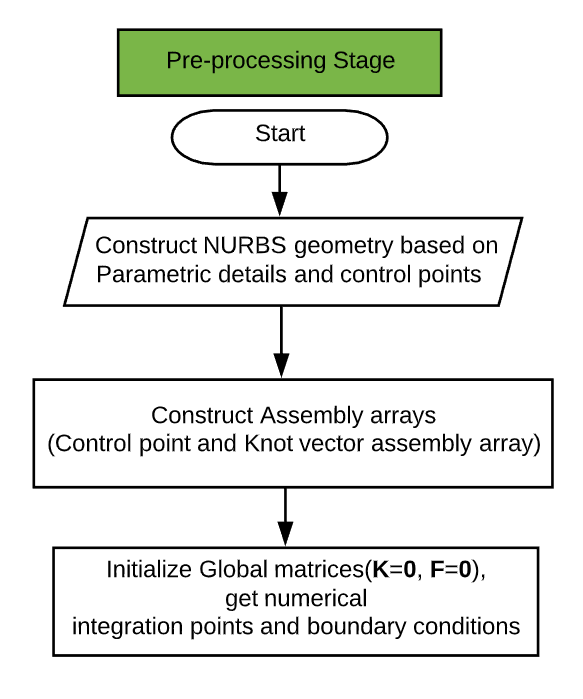
\includegraphics[scale=0.4]{PreProcessing.png} 
		\caption{\\Flow chart describing Pre-processing Stage of IGA}\label{PreProcessing}
	\end{center}
	
\end{figure}
\subsection{Pre-processing Stage of the Analysis}
This subsection mainly deals with NURBS based geometry creation, types of assembly arrays needed to assemble discretized geometries and how to deal with homogeneous and non-homogeneous boundary conditions on boundary defining control points due to their higher ($C^{p-1}$) continuity unlike $C^{0}$ continuity of FEM nodes.

\subsubsection{Geometry Creation} \label{GeometryCreation}
As mentioned before in the section \ref{NURBS}, apart from the physical details of the geometry like length, width and thickness etc. the construction of NURBS discretized geometry requires parametric details such as control points, knot vectors and the order of the NURBS curve. Commercial software like "Rhino" can be used to extract parametric details of the complex NURBS geometry. \\ The following function in python is used for finding a point on the NURBS surface.
\begin{verbatim}
NURBS_Surface_Point(n,p,U,m,q,V,Pw,u,v)
\end{verbatim}
Where, p and q are the degrees of the NURBS curve in $\xi$ and $\eta$ directions respectively, Pw control points vector, U and V are knot vectors in $\xi$ and $\eta$ directions respectively. 
n and m are calculated using below code
\begin{verbatim}
n=(np.size(U)-1)-p-1
m=(np.size(V)-1)-q-1 
\end{verbatim}
u and v are any points in knot span, for example if 
$U = \{0,0,1,2,3,4,4\}$,
u can be 2.5 which belongs to knot span $\{2,3\}$ in U.\\
The entire surface can be generated by looping over knot span points and by extracting surface points by using the above function and plotting the output. 
An example output of the geometry generated with the written code is shown below
\begin{figure}[H]
	\begin{center}
		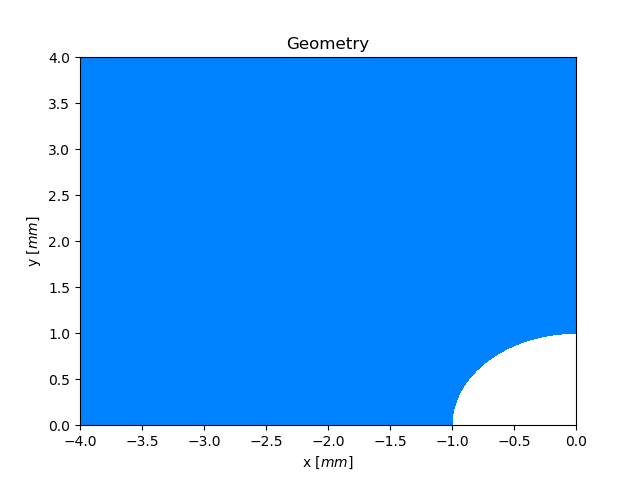
\includegraphics[scale=0.6]{Geometry.png} 
		\caption{\\NURBS Geometry}\label{Geometry}
	\end{center}	
\end{figure}
Parametric details of the geometry \cite{agrawal2019iga}:
\begin{verbatim}
Pw=
[[-1.,0.,0.,1],[-0.85,0.35,0.,0.85],[-0.35,0.85,0.,0.85],[0.,1.,0.,1]],
[[-2.5,0.,0.,1.],[-2.5,0.75,0.,1.],[-0.75,2.5,0.,1.],[0.,2.5,0.,1.]],
[[-4,0.,0.,1.],[-4,4.,0.,1.],[-4.,4.,0.,1.],[0.,4.,0.,1.]]
p=2 and q=2 # Degree of the curve in xi and eta directions
U = [0., 0., 0., 1., 2., 2., 2.]
V = [0., 0., 0., 1., 1., 1.]
\end{verbatim}


 

\subsubsection{Assembly arrays} \label{AssemblyArrays}
Assembly arrays are required to assemble local discretized geometries to global geometry. For IGA, as knot vector and control points define the geometry, two assembly arrays (1) Control point assembly array and (2) Knot vector connectivity array are required.
\begin{enumerate}[leftmargin=*]
	\item Control point assembly array: \\
	The degree of the NURBS curve determines the number of control points ($n^e_{cp}$) present in an IGA element.
	Considering a two-dimensional element ($\Omega^e$)\\
	$n^e_{cp}$ = $(p+1)(q+1)$ \\
	The details of the control points are stored row wise in assembly array.
	The following function generates a control point assembly array
	\begin{verbatim}
	def ControlPointAssembly(n,p,m,q,ele_no):
	
	#-----------------Inputs-----------------------#
	# n-no.of control points along xi direction
	# p-Degree of basis function along xi direction
	# m-no.of control points along eta direction
	# q-Degree  of basis function along eta direction
	#-----------------Output-----------------------#
	CP - Control point assembly array
	\end{verbatim}
	A control point assembly contains a two-dimensional array with control point numbers of each element, row-wise.
	An assembly array with 2 elements, as in Fig. (\ref{Element}) is shown below
	\begin{equation} \label{CPassembly}
	\textbf{CP} =
	\begin{bmatrix}
		1 & 2 & 4 & 5 \\
		2 & 3 & 5 & 6 \\
	\end{bmatrix}
	\end{equation}
	\begin{figure}[H]
		\begin{center}
			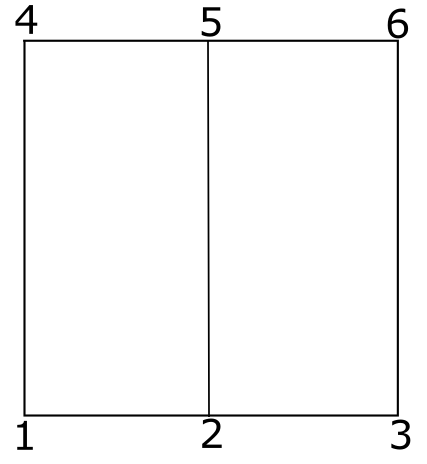
\includegraphics[scale=0.2]{Element.png} 
			\caption{\\A simple 2D square geometry with two elements}\label{Element}
		\end{center}	
	\end{figure}
	\item Knot vector connectivity array: \\
	The knot vector connectivity matrix \textbf{CP} is a row-wise matrix with each row corresponds to the respective element. The columns correspond to span ranges (Span$\_$U and Span$\_$V) along $\xi$ and $\eta$ directions. \\
	Knot vector array along $\xi$ and $\eta$ direction for geometry, Fig.(\ref{Element}): \\
	$U = [ 0, 0, 1, 2, 2 ]$ \\
	$V = [ 0, 0, 1, 1 ]$ \\
	Span$\_$U is a 2D array which has rows equal to number of elements in $\xi$ direction.
	\begin{equation} \label{SpanU}
	\textbf{Span\_U} =
	\begin{bmatrix}
	0 & 1  \\
	1 & 2  \\
	\end{bmatrix}
	\end{equation}
	Similarly with only one element along $\eta$ direction
	\begin{equation} \label{SpanU}
	\textbf{Span\_V} =
	\begin{bmatrix}
	0 & 1  \\
	\end{bmatrix}
	\end{equation}
	Knot connectivity for above geometry is given by,
	\begin{equation} \label{CP}
	\textbf{CP} =
	\begin{bmatrix}
	1 & 1  \\
	2 & 1  \\
	\end{bmatrix}
	\end{equation}
\\
	The following lines of code executes Knot Connectivity array
	\begin{verbatim}
	uniqueU = np.unique(U)
	uniqueV = np.unique(V)
	nelU = ncpxi-p
	nelV = ncpeta-q
	CP = np.zeros((nel,2)) 
	Span_U=np.zeros((nelU,2))#Span_U have rows equal to number of elements in xi direction
	Span_V=np.zeros((nelV,2))#Span_V have rows equal to number of elements in eta direction
	count=0
	for i in range(0,nelV):
	for j in range(0,nelU):
	CP[count,:] = [j+1,i+1] 
	# First and second coloumns of 'knotConnectivity' store the global number of knot 
	span ranges
	# or row number of Span_U and Span_V arrays
	Span_U[j,:]= [uniqueU[j],uniqueU[j+1]]
	Span_V[i,:]= [uniqueV[i],uniqueV[i+1]]
	count=count+1
	CP = knotConnectivity -1
	CP = CP.astype(int)
	\end{verbatim} 
	
	
	\begin{verbatim}

	\end{verbatim}
\end{enumerate}
\subsubsection{Boundary Conditions}
A brief description of how to define boundary conditions (BCS) is described in this section. When the order of the NURBS curve is two in each direction, a traditional way of defining homogeneous and inhomogeneous boundary conditions as in FEM can be followed. In any other case, a special treatment for defining BCS have to be followed, which is not in the scope of this project. Procedures like the least square minimization method are usually adopted for this purpose. 


\subsection{Processing Stage of the Analysis} \label{ProcessingStage}
In the processing stage of analysis, it is required to compute the global elemental stiffness matrix and global force vector and solve these for the solution field. To formulate the matrices, it requires NURBS basis functions and their derivatives evaluation. A numerical integration scheme, like the Gauss-Legendre rule, is employed to solve the volume and area integrals involved in forming the stiffness matrix and internal force vector. Numerical integration involves mapping elements from physical space to master space (which is also called the unit domain). As NURBS basis functions are defined in parametric space as given in Eq. (\ref{NURBSBasisFuncs})it requires an additional mapping from physical space to parametric space ($\Omega_e \rightarrow \widetilde{\Omega_e}$). Later parametric space can be mapped on to master space (($\widetilde{\Omega_e} \rightarrow \overline{\Omega_e}$)). This procedure is illustrated in Fig.(\ref{MasterPhysical}).
\begin{figure}[H]
	\begin{center}
		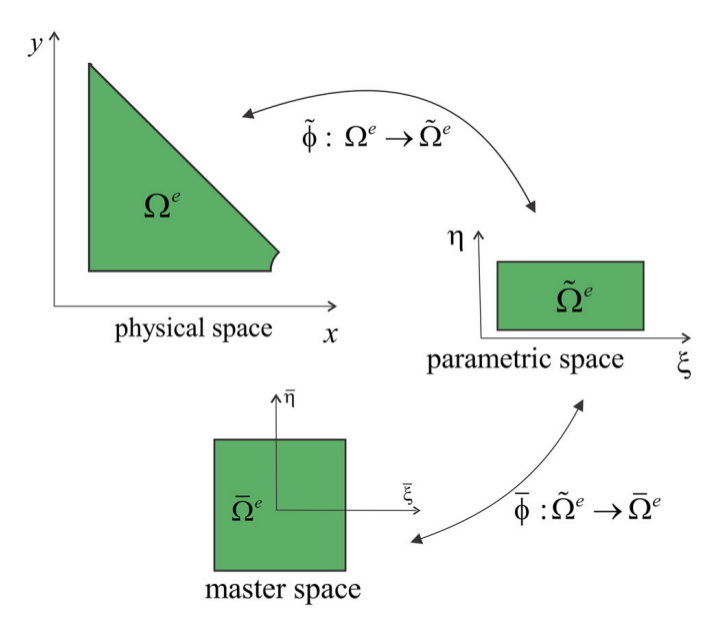
\includegraphics[scale=0.3]{Physical_Master.png} 
		\caption{\\Mapping IGA Physical element to Master
			element \cite{agrawal2019iga}}\label{MasterPhysical}
	\end{center}	
\end{figure}


\begin{enumerate}[leftmargin=*]
	\item Mapping from master space to parametric space \cite{agrawal2019iga}: \\
	Consider a discretized IGA surface which is defined in parametric space
	$\widetilde{\Omega_e}=[\xi_i,\xi_{i+1}]\otimes[\eta_i,\eta_{i+1}]$, Refer
	Fig.(\ref{MasterPhysical}). The NURBS basis functions and their derivatives are evaluated at
	$\xi,\eta$ of the element $\widetilde{\Omega_e}$. These $\xi,\eta$ co-ordinate
	values are calculated by a linear mapping as shown below
	\begin{equation}
	\xi=\frac{1}{2}[(\xi_{i+1}-\xi_{i})\overline{\xi}+(\xi_{i+1}+\xi_{i})]
	\end{equation} 
	\begin{equation}
	\eta=\frac{1}{2}[(\eta_{i+1}-\eta_{i})\overline{\eta}+(\eta_{i+1}+\eta_{i})]
	\end{equation}
	where $\overline{\xi},\overline{\eta}$ are the integration points defined in
	master space \\
	$\textbf{J}_2$ matrix is defined as 
	\begin{equation}
	\textbf{J}_2 = \frac{\partial\xi}{\partial \bar{\xi}}
	\frac{\partial\eta}{\partial \bar{\eta}}
	\end{equation} 
	Determinant of $\textbf{J}_2$ matrix is required in numerical integration
	scheme for linear mapping 
	
	
	\item Mapping from physical space to parametric space \cite{agrawal2019iga}: \\
	The Jacobian matrix $\textbf{J}_1$ used to map from physical space to
	parametric space ($\Omega_e \rightarrow \widetilde{\Omega_e}$) is computed as:
	
	\begin{equation} \label{J1Matrix1}
	\textbf{J}_1 =
	\large
	\begin{bmatrix}
	\frac{\partial x}{\partial \xi} &\frac{\partial x}{\partial \eta} \\
	\frac{\partial y}{\partial \xi} &\frac{\partial y}{\partial \eta} \\
	\end{bmatrix} 
	\end{equation}
	
	The components of the $\textbf{J}_1$ matrix are calculated using Eq.
	(\ref{Co-ordinate}).
	
	\begin{equation}
	\frac{\partial x}{\partial \xi} = \sum_{k=1}^{n_{cp}^e} \frac{\partial
		\textbf{R}_k}{\partial \xi} x_i
	\qquad
	\frac{\partial x}{\partial \eta} = \sum_{k=1}^{n_{cp}^e} \frac{\partial
		\textbf{R}_k}{\partial \eta} x_i
	\end{equation} 
	
	\begin{equation}
	\frac{\partial y}{\partial \xi} = \sum_{k=1}^{n_{cp}^e} \frac{\partial
		\textbf{R}_k}{\partial \xi} y_i
	\qquad
	\frac{\partial y}{\partial \eta} = \sum_{k=1}^{n_{cp}^e} \frac{\partial
		\textbf{R}_k}{\partial \eta} y_i
	\end{equation}
	
\end{enumerate}
The two different mappings described above can be illustrated with an example
considering $ \textbf{F}(x,y)$ integrated over the physical space $\Omega$

\begin{equation*}
\begin{split}
\int_{\Omega} \textbf{F}(x,y)d\Omega & = \sum_{e=1}^{nel} \int_{\Omega_e}
\textbf{F}(x,y) d\Omega  \\
& = \sum_{e=1}^{nel} \int_{\widetilde{\Omega_e}}
\textbf{F}(\xi,\eta)|\textbf{J}_1| d\xi d\eta \\
& = \sum_{e=1}^{nel} \int_{\overline{\Omega_e}}
\textbf{F}(\overline\xi,\overline\eta)|\textbf{J}_1||\textbf{J}_2| d\overline\xi
d\overline\eta  \\
& = \sum_{e=1}^{nel} \int_{-1}^{1} \int_{-1}^{1}
\textbf{F}(\overline\xi,\overline\eta)|\textbf{J}_1||\textbf{J}_2| d\overline\xi
d\overline\eta  \\
& = \sum_{e=1}^{nel} \left[ \sum_{i=1}^{n_{gp}^e}
\textbf{F}(\overline\xi_i,\overline\eta_i) gw_i |\textbf{J}_1||\textbf{J}_2|
d\overline\xi d\overline\eta \right]
\end{split}
\end{equation*}

\noindent
where $nel$ is the total number of elements and $n_{gp}^e$, $gw_i$ denotes the
number of Gauss points and their respective Gauss weights.\\
\noindent
The following function is used to get the J1 and J2 matrix along with their determinants.
\begin{verbatim}
--------------------------------------------------------------
def Jacobian12(xi,eta,elU,elV):
#-----------------Input------------------#
Parametric Co-ordinates (xi,eta) of Gauss Points
Knot span range (elU,elV) in xi and eta direction
#-----------------Output-----------------#
J1 and J2 matrices along with their determinants
--------------------------------------------------------------
\end{verbatim}
The formulated global stiffness matrix and force vector are solved using a numerical scheme like the Newton-Raphson method for the solution field.
\\A flow chart describing processing stage flow is shown in Fig.(\ref{Processing})
\begin{figure}[H]
	\begin{center}
		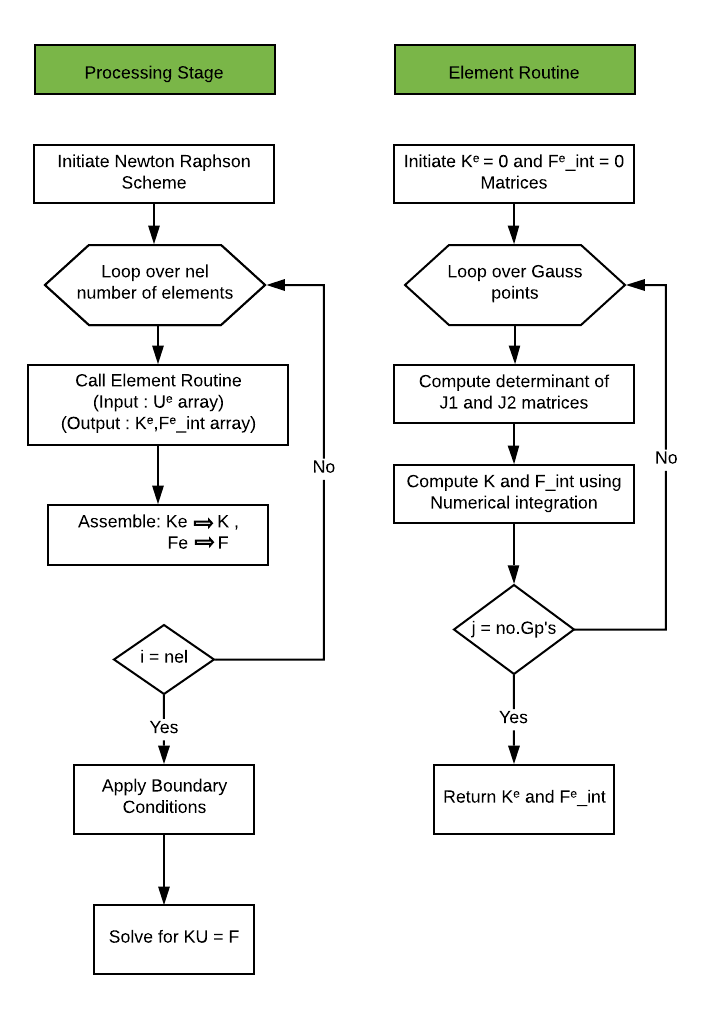
\includegraphics[scale=1.0]{Processing.png} 
		\caption{\\Flow chart describing Processing Stage of IGA}\label{Processing}
	\end{center}
\end{figure}

\subsection{Post-processing Stage of the Analysis}
This section deals with the visualization of the deformed geometry and how a
displacement and solution dependent variables are plotted. 

\begin{enumerate}[leftmargin=*]
	\item Visualization of the deformed NURBS geometry:	
	
	Visualization of the deformed geometry can be done in the same manner as the visualization of the initial geometry. After determining the displacement field at the control points, they are added to the initial control points coordinates
	$[\textbf{P}]$.\\
	\\
	$[\textbf{P}_{new}]=[\textbf{P}]+[\textbf{U}]$ \\
	\\
	$[\textbf{P}_{new}]$ control points array is used to plot the deformed
	geometry.
	As discussed in section (\ref{GeometryCreation}), instead of initial control point matrix of the geometry \textbf{P}, \textbf{$P_{new}$} is given as input to the function 
	\begin{verbatim}
	def NURBS_Surface_Point(n,p,U,m,q,V,P_new,u,v):
	\end{verbatim}
	and the deformed geometry can be plotted.
	 
	
	\item Plotting of displacements and solution dependent variables:
	
	A contour plot can be made using the displacement values ($U$) on deformed or undeformed geometry.
	Due to the higher continuity of the NURBS basis functions, stress recovery techniques are not necessary to extract the solution field on the deformed geometry.  
	
	\textbf{plt.contourf} a matplotlib function is used to plot displacements, reaction forces, and electrical potentials, so that the comparison with Abaqus post-processing plots would be easier. The latter plots the solution fields as a contour plot.
	
\end{enumerate}

\begin{figure}[H]
	\begin{center}
		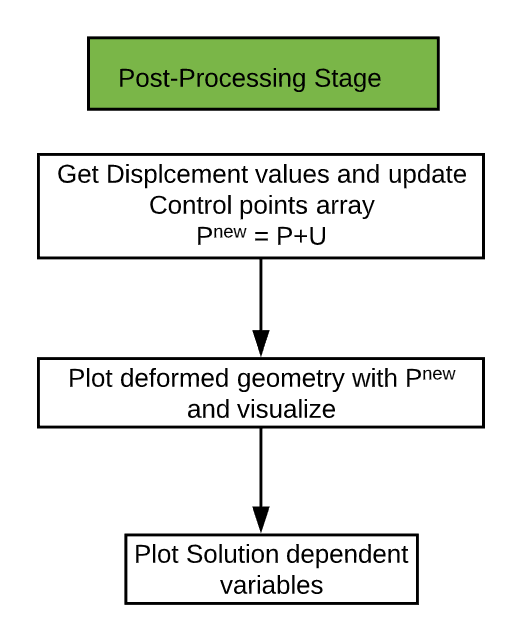
\includegraphics[scale=0.5]{PostProcessing.png} 
		\caption{\\Flow chart describing Post-processing Stage of IGA}\label{PostProcessing}
	\end{center}
	
\end{figure}

\newpage
\section{Mechanical Case}


\subsection{Governing Equations}
The governing equation for mechanical deformation is based on conservation of
linear momentum which can be written as
\begin{equation}\label{ConservationOfLM}
\sigma_{ij,i} + b_j = 0
\end{equation}
where $ \sigma_{ij} $ and $ b_i $ is the Cauchy stress tensor and the body force.
Due to the static nature of the analysis, the inertial term is not included in
the eq(\ref{ConservationOfLM}).\\*
Stress and strain are related by following constitutive equation
\begin{equation}
\sigma_{ij} = c_{ijkl} \epsilon_{kl}
\end{equation}
The infinitesimal strain theory is adopted for the analysis in which
displacements of the material particles are considered to be very small compared
to the dimensions of the body under loading. Strain in a small strain setting
can be written as
\begin{equation}
\epsilon_{ij}=\frac{1}{2}[u_{i,j}+u_{j,i}]
\end{equation}
where $ u_{i} $ are the displacements in the body


\subsection{Weak Formulation}
Consider a domain $\Omega$ with $\Gamma_u$ as prescribed displacements and
$\Gamma_t$ as traction boundary conditions. The domain boundary can be
represented as $\Gamma = \Gamma_u \cup \Gamma_t$ and $\Gamma_u \cap \Gamma_t =
\Phi$
By using the principle of virtual work the eq(\ref{ConservationOfLM}) can be written as
\begin{equation}
\delta W = \int_\Omega (\sigma_{ij,i} + b_j ) \delta u_j dV = 0
\end{equation} 
with,
$u = u_o$ on $\Gamma_u$ (essential boundary condition) and
$\sigma_{ij}n_j = \bar{t}_j$ on $\Gamma_t$ (natural boundary condition) \\*
where $\delta u_j$ is the virtual displacement field, $n_j$ is unit normal to
the surface \\*
Applying integration by parts to the stress term under integral and by making
using of conservation of angular momentum ($ \sigma_{ij} = \sigma_{ji} $) and
Gauss divergence theorem (converting volume integral to surface integral) we
approach at the following equation
\begin{equation} \label{FinalWeakform}
\delta W = \int_{\Omega} \sigma_{ij} \epsilon_{ij} d\Omega - \left[
\int_{\Gamma} \bar{t}_j \delta u_j d\Gamma_t  + \int_{\Omega} b_j \delta u_j
d\Omega \right]
\end{equation}
as an additional requirement $\delta u_j$ must be zero at the essential boundary
conditions ($\Gamma_u$) for a unique solution.


\subsection{IGA Formulation}
The advantage of IGA over FEM formulation lies in its basis functions
incorporation and its ability to capture the exact geometry. While the FEM uses lagrangian basis functions, IGA uses NURBS basis functions, which are used to generate the geometry itself. As discussed in the previous sections, a multidimensional NURBS basis function is represented by
$R_{i,j,k}^{p,q,r}(\xi,\eta,\zeta) \rightarrow R_i$. The isogeometric element 
is represented by basis function $R_i$ and control points $P_i$ as \cite{agrawal2019iga}
\begin{equation} \label{Co-ordinate}
\textbf{x}^e = \sum_{i=1}^{n_{cp}^e} R_i P_i
\end{equation} 
By Galerkin approach, the displacements and virtual displacements are given by
\begin{equation} \label{u_and_du}
\textbf{u}^e = \sum_{i=1}^{n_{cp}^e} R_i \textbf{u}_i \qquad \delta\textbf{u}^e
= \sum_{i=1}^{n_{cp}^e} R_i \delta\textbf{u}_i
\end{equation}
where $\textbf{u}_i$ and $\delta\textbf{u}_i$ are values at $i$th control point.
The strain displacement matrix \textbf{B} is given by
\begin{equation} \label{BMatrix}
\textbf{B} =
\begin{bmatrix}
R_{1,x} & 0 & 0 & R_{2,x} & 0 & 0 & .... & R_{n_{cp}^e,x} & 0 & 0 \\
0 &R_{1,y} & 0 & 0 & R_{2,y} & 0 & .... & 0 & R_{n_{cp}^e,y} & 0  \\
0 & 0 & R_{1,z} &0 & 0 & R_{2,z} & .... &0 & 0 & R_{n_{cp}^e,z}  \\
R_{1,y} & R_{1,x} & 0 & R_{2,y} & R_{2,x} & 0 & .... & R_{n_{cp}^e,y} &
R_{n_{cp}^e,x} & 0 \\
0 & R_{1,z} & R_{1,y} & 0 & R_{2,z} & R_{2,y} & .... & 0 & R_{n_{cp}^e,z} &
R_{n_{cp}^e,y}\\
R_{1,z} &0 & R_{1,x} & R_{2,z} &0 & R_{2,x} & .... &R_{n_{cp}^e,z} &0
&R_{n_{cp}^e,x}
\end{bmatrix}
\end{equation}
By substituting Eqs, (\ref{u_and_du}) and (\ref{BMatrix}) in
Eq.(\ref{FinalWeakform}), the weak form in matrix terms can be written as
\begin{equation} \label{MatrixWeakForm}
\sum_{e=1}^{nel} \left[ \left( \int_{\Omega_e} \textbf{B}^T \textbf{C}
\textbf{B} d\Omega \right) \right] \textbf{u} = \int_{\Gamma^e_t}
\textbf{R}^T.\textbf{t} d\Gamma + \int_{\Omega^e_t} \textbf{R}^T.\textbf{f}
d\Omega 
\end{equation}
where \text{R} is defined as \\
for the boundary $\Gamma^e$ 
\begin{equation} \label{RMatrix1}
\textbf{R} =
\begin{bmatrix}
R_1(\xi,\eta) & 0 & R_2(\xi,\eta) &0 & .... & R_{n_{cp}^e}(\xi,\eta) & 0 \\
0 &R_1(\xi,\eta) & 0 & R_2(\xi,\eta) & .... & 0 & R_{n_{cp}^e}(\xi,\eta) \\
\end{bmatrix}
\end{equation}
for the domain $\Omega^e$
\begin{equation} \label{RMatrix2}
\textbf{R} =
\begin{bmatrix}
R_1(\xi,\eta,\zeta) & 0 & R_2(\xi,\eta,\zeta) &0 & .... &
R_{n_{cp}^e}(\xi,\eta,\zeta) & 0 \\
0 &R_1(\xi,\eta,\zeta) & 0 & R_2(\xi,\eta,\zeta) & .... & 0 &
R_{n_{cp}^e}(\xi,\eta,\zeta) \\
\end{bmatrix}
\end{equation}
Eq.(\ref{MatrixWeakForm}) can be rewritten in a standard matrix form as
\begin{equation}
\sum_{e=1}^{nel} [\textbf{K}^e \textbf{U}^e = \textbf{F}^e] 
\end{equation}
where $\textbf{K}^e$ is isogeometric element’s stiffness matrix, $\textbf{U}^e$
is displacement vector and $\textbf{F}^e$ force vector



\newpage

\section{Piezoelectric Case}


\subsection{Governing Equations for Piezoelectric Materials}
The coupled electro-mechanical interactions are governed by conservation of
momentum and Gauss's law as \cite{nguyen2018finite}:
\begin{equation} \label{MechEq}
\sigma_{ij,j} + f_i = 0
\end{equation} 
\begin{equation} \label{ElecEq}
D_{i,i} - q = 0
\end{equation}
Where, $ f_i $ is body force, $ q $ is electrical charge, $ \sigma_{ij} $ is
Cauchy stress tensor and $ D_i $ is electrical displacement vector.
The constitutive equations for electromechanical coupling are defined as
\begin{equation}
\sigma_{ij} = C_{ijkl} \varepsilon_{kl} - e_{kij} E_k
\end{equation}
\begin{equation}
D_i = e_{ikl} \varepsilon_{kl} + \kappa_{ik} E_k
\end{equation}
Where, $ C $ , $ e $ and $ \kappa $ are elastic,
piezoelectric and dielectric material constants respectively. The Cauchy strain
tensor is defined as:
\begin{equation}
\varepsilon_{ij} = \frac{1}{2} (u_{i,j} + u_{j,i})
\end{equation}
and electric field vector as:
\begin{equation}
E_i = -\phi_{,i}
\end{equation}


\subsection{Weak Formulation}
Applying the principle of virtual work to the Eq.(\ref{MechEq})
and Eq. (\ref{ElecEq}) we can write \cite{nguyen2018finite}
\begin{equation} \label{CouplingWeakForm1}
\int_\Omega ( \sigma_{ij,j} + f_i ) \delta u_i d\Omega = 0  
\end{equation}
\begin{equation} \label{CouplingWeakForm2}
\int_\Omega (D_{i,i} - q ) \delta \phi d\Omega = 0
\end{equation}
with, \\
essential boundary conditions:
$u = u_o$ on $\Gamma_u$ and $\Phi=\Phi_0$ on $\Gamma_\Phi$ \\
natural boundary condition:
$\sigma_{ij}n_j = \bar{t}_j$ on $\Gamma_t$ and $D_i n_i = q_0$ on $\Gamma_q$ \\*
where $\delta u_i$ and $\delta \phi$ are virtual or arbitrary displacement and
potential fields. \\
Integrating Eq. (\ref{CouplingWeakForm1}) and Eq. (\ref{CouplingWeakForm2}) by
parts and later applying Gauss divergence theorem and boundary conditions we
approach at weak form
\begin{equation} \label{FinalCouplingWeakForm1}
\int_\Omega \sigma_{ij} \delta \epsilon_{ij} d\Omega - \left[ \int_{\Gamma}
\bar{t_i} \delta u_i d\Gamma + \int_\Omega f_i \delta u_i d\Omega  \right]= 0 
\end{equation}
\begin{equation} \label{FinalCouplingWeakForm2}
\int_\Omega D_i \delta E_i d\Omega - \left[ \int_{\Gamma} Q \delta \phi d\Gamma
+ \int_\Omega q \delta \phi d\Omega \right] = 0
\end{equation}


\subsection{IGA Formulation}
By Galerkin approach, displacements, potentials and their virtual values are
given by below equations \cite{agrawal2019iga}

\begin{equation} \label{u_and_du_2}
\textbf{u}^e = \sum_{i=1}^{n_{cp}^e} R_i \textbf{u}_i \qquad \delta\textbf{u}^e
= \sum_{i=1}^{n_{cp}^e} R_i \delta\textbf{u}_i
\end{equation}

\begin{equation} \label{Phi_and_dPhi_2}
\Phi^e = \sum_{i=1}^{n_{cp}^e} R_i \Phi_i \qquad \delta\Phi^e =
\sum_{i=1}^{n_{cp}^e} R_i \delta\Phi_i
\end{equation}

\noindent
where $\textbf{u}_i$ , $\delta\textbf{u}_i$, $\delta\Phi_i$ and $\Phi_i$ are
values at $i$th control point.\\
By substituting Eqs, (\ref{u_and_du_2}) and (\ref{Phi_and_dPhi_2}) in
Eq.(\ref{FinalCouplingWeakForm1}) and Eq.(\ref{FinalCouplingWeakForm2}) the weak
form in matrix notation can be written as

\begin{equation} \label{CoupledStiffnessMatrix}
\begin{bmatrix} 
K_{MM} & K_{ME} \\
K_{EM} & K_{EE} \\ 
\end{bmatrix}
\begin{bmatrix} 
\textbf{u} \\
\phi \\ 
\end{bmatrix} = \begin{bmatrix} 
F_M \\
F_E \\ 
\end{bmatrix}
\end{equation}  
Where,
\begin{equation}
K_{MM} = \int_\Omega \textbf{B}_u^T \textbf{C} \textbf{B}_u d\Omega
\end{equation}
\begin{equation}
K_{ME} = \int_\Omega \textbf{B}_u^T \textbf{e} \textbf{B}_e d\Omega
\end{equation}
\begin{equation}
K_{EM} = \int_\Omega \textbf{B}_e^T \textbf{e}^T \textbf{B}_u d\Omega
\end{equation}
\begin{equation}
K_{EE} = - \int_\Omega \textbf{B}_e^T \kappa \textbf{B}_e d\Omega
\end{equation}
\begin{equation}
F_M = \int_\Omega \textbf{R}_u^T \textbf{f} d\Omega + \int_\Gamma \textbf{R}_u^T
\textbf{t} d\Gamma 
\end{equation}
\begin{equation}
F_E = \int_\Omega \textbf{R}_e^T q d\Omega + \int_\Gamma \textbf{R}_e^T Q
d\Gamma 
\end{equation}

\noindent
where \text{R} is defined as \\
for the boundary $\Gamma$ 

\begin{equation} \label{RMatrix11}
\textbf{R}_u =
\begin{bmatrix}
R_1(\xi,\eta) & 0 & R_2(\xi,\eta) &0 & .... & R_{n_{cp}^e}(\xi,\eta) & 0 \\
0 &R_1(\xi,\eta) & 0 & R_2(\xi,\eta) & .... & 0 & R_{n_{cp}^e}(\xi,\eta) \\
\end{bmatrix}
\end{equation}

\begin{equation} \label{RMatrix12}
\textbf{R}_e =
\begin{bmatrix}
R_1(\xi,\eta) & R_2(\xi,\eta) & .... & R_{n_{cp}^e}(\xi,\eta) \\
\end{bmatrix}
\end{equation}

\noindent
for the domain $\Omega$

\begin{equation} \label{RMatrix21}
\textbf{R}_u =
\begin{bmatrix}
R_1(\xi,\eta,\zeta) & 0 & R_2(\xi,\eta,\zeta) &0 & .... &
R_{n_{cp}^e}(\xi,\eta,\zeta) & 0 \\
0 &R_1(\xi,\eta,\zeta) & 0 & R_2(\xi,\eta,\zeta) & .... & 0 &
R_{n_{cp}^e}(\xi,\eta,\zeta) \\
\end{bmatrix}
\end{equation}

\begin{equation} \label{RMatrix22}
\textbf{R}_e =
\begin{bmatrix}
R_1(\xi,\eta,\zeta) & R_2(\xi,\eta,\zeta) & .... & R_{n_{cp}^e}(\xi,\eta,\zeta)
\\
\end{bmatrix}
\end{equation}

\noindent
B matix is given as

\begin{equation} \label{BuMatrix}
\textbf{B}_u =
\begin{bmatrix}
R_{1,x} & 0 & 0 & R_{2,x} & 0 & 0 & .... & R_{n_{cp}^e,x} & 0 & 0 \\
0 &R_{1,y} & 0 & 0 & R_{2,y} & 0 & .... & 0 & R_{n_{cp}^e,y} & 0  \\
0 & 0 & R_{1,z} &0 & 0 & R_{2,z} & .... &0 & 0 & R_{n_{cp}^e,z}  \\
R_{1,y} & R_{1,x} & 0 & R_{2,y} & R_{2,x} & 0 & .... & R_{n_{cp}^e,y} &
R_{n_{cp}^e,x} & 0 \\
0 & R_{1,z} & R_{1,y} & 0 & R_{2,z} & R_{2,y} & .... & 0 & R_{n_{cp}^e,z} &
R_{n_{cp}^e,y}\\
R_{1,z} &0 & R_{1,x} & R_{2,z} &0 & R_{2,x} & .... &R_{n_{cp}^e,z} &0
&R_{n_{cp}^e,x}
\end{bmatrix}
\end{equation}

\begin{equation} \label{BeMatrix}
\textbf{B}_e =
\begin{bmatrix}
R_{1,x} & R_{2,x} & .... & R_{n_{cp}^e,x} \\
R_{1,y} & R_{2,y} & .... & R_{n_{cp}^e,y} \\
R_{1,z} & R_{2,z} & .... & R_{n_{cp}^e,z} \\
\end{bmatrix}
\end{equation}

\begin{equation}
\varepsilon = \textbf{B}_u . \textbf{u}
\end{equation}

\begin{equation}
\textbf{E} = - \textbf{B}_e . \Phi
\end{equation}

\noindent
Eq. (\ref{CoupledStiffnessMatrix}) can be solved using numerical methods like
Newton-Raphson method for displacements and potential solution fields.

\newpage
\section{Modelling and Results}
\subsection{2D Plate with linear elastic loading} 
\subsubsection{Problem description} \label{2DPWLELPD}
A 2D plate is subjected to mechanical loading as shown in Figure(\ref{XYLoading}). The material used is PZT-PIC151 ceramics \cite{kozinov2018simulation}, and the elastic constants of the material are given in the appendix (\ref{MaterialProps}).
The movement of bottom edge AB is fixed in y-direction and left edge AC in x-direction. A displacement of 0.1 mm is given on the right edge BD.
\begin{figure}[H]
	\centering
	\begin{minipage}{.5\textwidth}
		\centering
		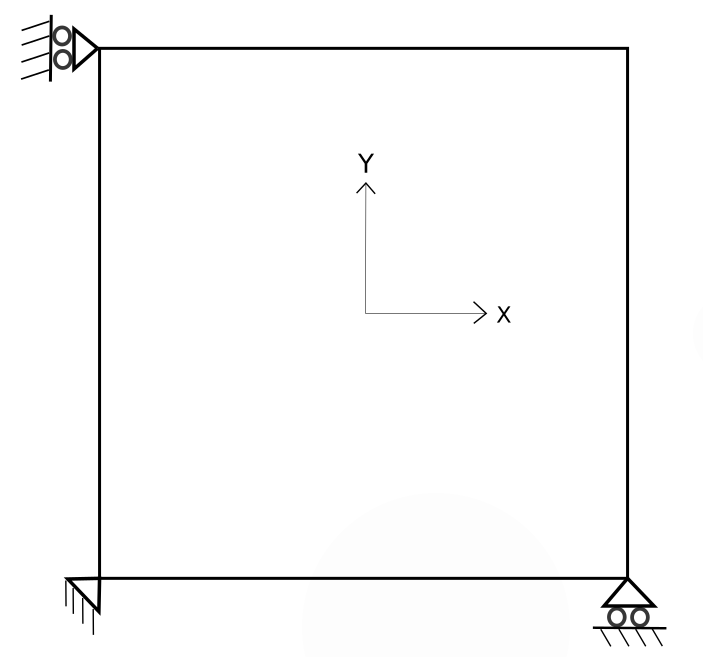
\includegraphics[width=0.8\linewidth]{2DPlate.png}
		\captionof{figure}{2D Plate}
		\label{2Dplate}
	\end{minipage}%
	\begin{minipage}{.5\textwidth}
		\centering
		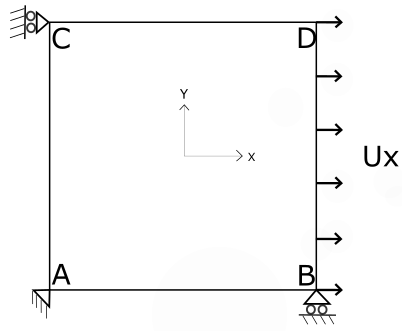
\includegraphics[width=0.9\linewidth]{XYLoading.png}
		\captionof{figure}{2D Plate with loading}
		\label{XYLoading}
	\end{minipage}
\end{figure}
\subsubsection{Parametric details for the plate with single element}
\label{ParametricDeatils1Elem}
The 2nd order NURBS curve is used in both $\xi$ and $\eta$ directions. \\
\begin{comment}
The knot vectors along $\xi$ and $\eta$ directions are \\
$\Xi= [0,0,1,1]$ and $\eta= [0,0,1,1]$. \\
Control points along $\xi$ direction is given by \\
$n_{cp}(\xi)$ = total number of knots in $[\Xi] - (p+1) = 2$.\\
Similarly the total number of control points along $\eta$ direction is given
by\\ $n_{cp}(\eta)$ = total number of knots in $[H ]- (q+1) = 2$ . \\
The total number of control points which defines the surface is\\
$n_{cp}$ = $n_{cp}(\xi) * n_{cp}(\eta)$ which is $2*2 = 4$. \\
\end{comment}
%\begin{verbatim}
\begin{enumerate}
	\item Physical details for the geometry: \\
	L = 10 \qquad \# Length of the plate in mm \\
	H = 10 \qquad \# Height of the plate in mm \\
	T =  1 {}  \qquad \# Thickness of the plate in mm \\
	
	\item Parametric details of the geometry: \\
	$\Xi$ = [0,0,1,1] \qquad \# Knot vector in $\xi$  direction \\
	$H$ = [0,0,1,1] \qquad \# Knot vector in $\eta$ direction \\
	
	Degree of the curve \\
	p=1 \qquad \# Degree of the curve in $\xi$  direction \\
	q=1 \qquad \# Degree of the curve in $\eta$ direction \\
	
	Number of control points in each direction \\
	$n_{cp}^{\xi}$  = len($\Xi$) - (p+1)  \qquad \#No.of control points in $\xi$
	direction (4-(1+1) = 2) \\
	$n_{cp}^{\eta}$ = len($H$) - (q+1)  \qquad \#No.of control points in $\eta$
	direction (4-(1+1) = 2) \\
	
	\item Total number of control points for the geometry \\
	$n_{cp} = n_{cp}^{\xi} * n_{cp}^{\eta}$ = 2*2 = 4\\
	\begin{comment}
	\item Control points net for the geometry \\
	P = [[[0,0,0,1],[L,0,0,1]],
	[[0,L,0,1],[L,L,0,1]]]
	
	$$
	P = \begin{bmatrix}
	[0,0,0,1] & [L,0,0,1] \\
	[L,0,0,1] & [L,L,0,1] \\
	\end{bmatrix} 
	$$
	
	\end{enumerate}
	%\end{verbatim}
	\end{comment}
	The control points are given by
	\begin{center}
		\begin{tabular}{ |c|c|c|c|c| } 
			\hline
			i & $ P_{i,0} $ & $ P_{i,1} $  \\ \hline
			0 & $ (0,0,0,1) $ & $ (0,10,0,1) $  \\ \hline
			1 & $ (10,0,0,1) $ & $ (10,10,0,1) $  \\ \hline
			
		\end{tabular}
	\end{center}
	with the fourth value in the parentheses being weights of respective control points.
	**As this is the case of single element, there is no need for the control point
	assembly array and knot vector connectivity matrix.
\end{enumerate}
\subsubsection{Results and discussions} \label{ResultsMech}
Considering the accuracy of the IGA simulation results over FEM results, IGA code generated results can be compared with the Abaqus inbuilt element generated results. An Abaqus plane strain full integration element (\textbf{CPE4}) \cite{abaqus10version} is used for this purpose.
\\The below figures show the values of displacements (U) and reaction forces (RF ) for both Abaqus and IGA element.\\

\textbf{**A similar contour is used for the program generated results and Abaqus results for easy comparison. }\\
Figure(\ref{M1U1}) and Figure(\ref{M1U1_IGA}) show the displacement (U1) values of the single CPE4 element and single IGA element at 100 \% loading in x-direction respectively. \\
\begin{figure}[H]
	\centering
	\begin{minipage}{.5\textwidth}
		\centering
		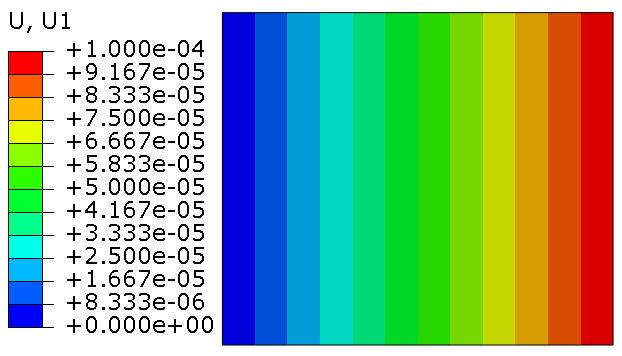
\includegraphics[width=1\linewidth]{M1U1.png}
		\captionof{figure}{CPE4 Element:U1 \\\textbf{Abaqus generated result}}
		\label{M1U1}
	\end{minipage}%
	\begin{minipage}{.5\textwidth}
		\centering
		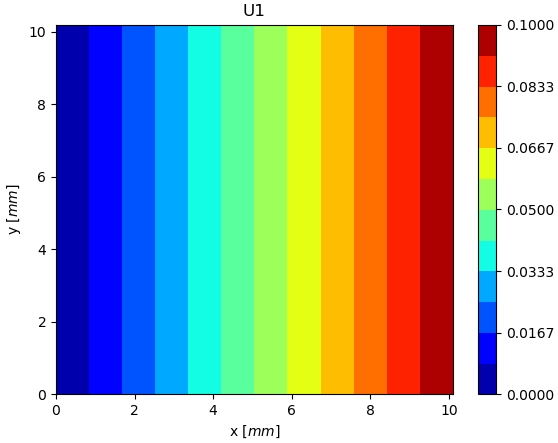
\includegraphics[width=1\linewidth]{M1U1_IGA.png}
		\captionof{figure}{IGA Element:U1 \\ \textbf{Program generated result}}
		\label{M1U1_IGA}
	\end{minipage}
\end{figure}
\begin{comment}
		\begin{figure}[H]
		\begin{center}
		\includegraphics[scale=0.45]{xyz.png} 
		\caption{\\CPE4 Element U1}\label{xyz}
		\end{center}	
		\end{figure}
		
		\begin{figure}[H]
		\begin{center}
		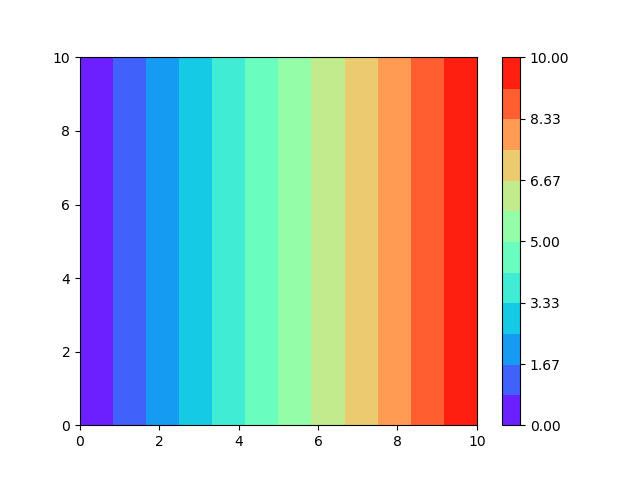
\includegraphics[scale=0.8]{Figure_1.png} 
		\caption{\\IGA Element U1}\label{Figure_1}
		\end{center}	
		\end{figure}
\end{comment}
Figure(\ref{M1U2}) and Figure(\ref{M1U2_IGA}) show the displacement (U2) values of the single CPE4 element and single IGA element at 100 \% loading in y-direction respectively. \\
\begin{figure}[H]
	\centering
	\begin{minipage}{.5\textwidth}
		\centering
		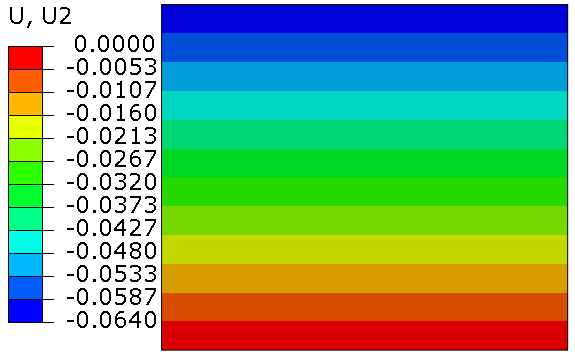
\includegraphics[width=1\linewidth]{M1U2.png}
		\captionof{figure}{CPE4 Element:U2
		\\\textbf{Abaqus generated result}}
		\label{M1U2}
	\end{minipage}%
	\begin{minipage}{.5\textwidth}
		\centering
		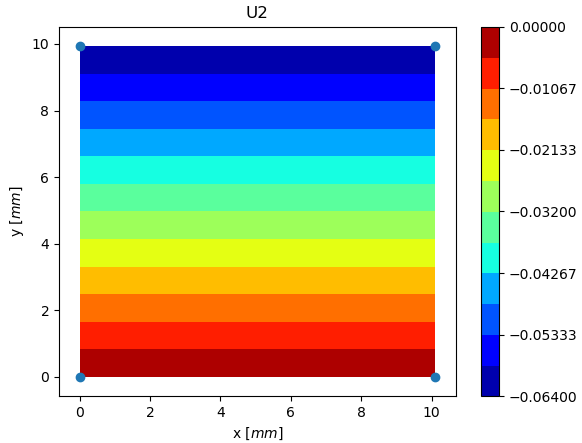
\includegraphics[width=1\linewidth]{M1U2_IGA.png}
		\captionof{figure}{IGA Element:U2\\ \textbf{Program generated result}}
		\label{M1U2_IGA}
	\end{minipage}
\end{figure}



Figure(\ref{M1RF1}) and Figure(\ref{M1RF1_IGA}) show the Reaction force values (RF1) of the single CPE4 element and single IGA element at 100 \% loading in x-direction respectively. \\
\begin{figure}[H]
	\centering
	\begin{minipage}{.5\textwidth}
		\centering
		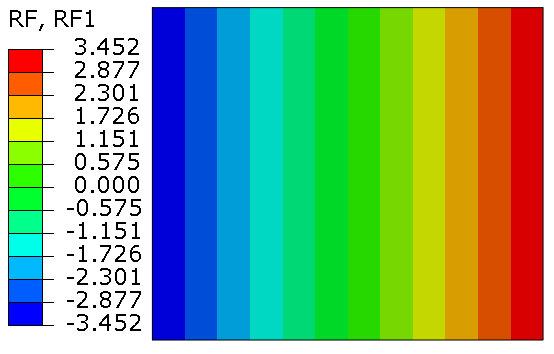
\includegraphics[width=1\linewidth]{M1RF1.png}
		\captionof{figure}{CPE4 Element:RF1
		\\\textbf{Abaqus generated result}}
		\label{M1RF1}
	\end{minipage}%
	\begin{minipage}{.5\textwidth}
		\centering
		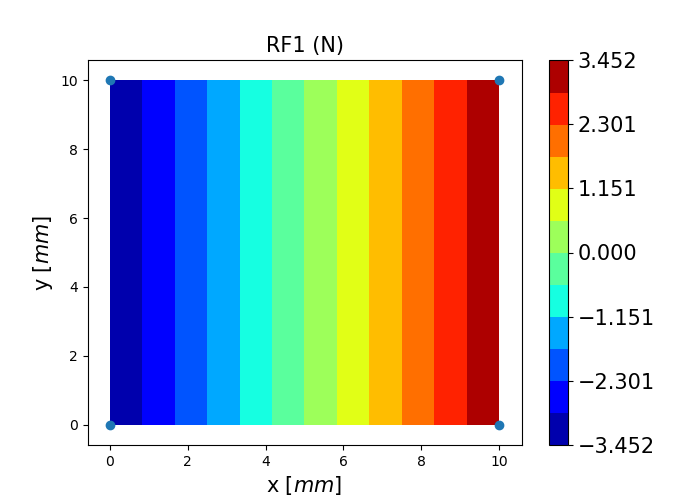
\includegraphics[width=1\linewidth]{M1RF1_IGA.png}
		\captionof{figure}{IGA Element:RF1\\ \textbf{Program generated result}}
		\label{M1RF1_IGA}
	\end{minipage}
\end{figure}

*** Reaction force in the y-direction is not reported since the loading is given only in the x-direction, and for the given fixed BCS, the RF2 is negligible.  \\

\subsubsection{Conclusion}
As shown in figures above the values generated by IGA code are in-line with the results of the Abaqus element. So it can be concluded that IGA code written works well with 2D one element case.






\subsection{2D Plate with pure Electrical loading}
\subsubsection{Problem description}\label{2DPWPELPD}
A 2D plate is subjected to Electrical loading as shown in Figure(\ref{PureElectrical22}).The material used is PZT-PIC151 ceramics, and the dielectric constants can be seen in Appendix (\ref{MaterialProps})
The movement of bottom edge AB is fixed in y-direction and left edge AC in x-direction.The top edge CD is grounded ( potential = 0 volts). An electrical potential V of 1000 volts is applied on bottom edge AB as shown in Fig. (\ref{PureElectrical22})
\begin{figure}[H]
	\centering
	\begin{minipage}{.4\textwidth}
		\centering
		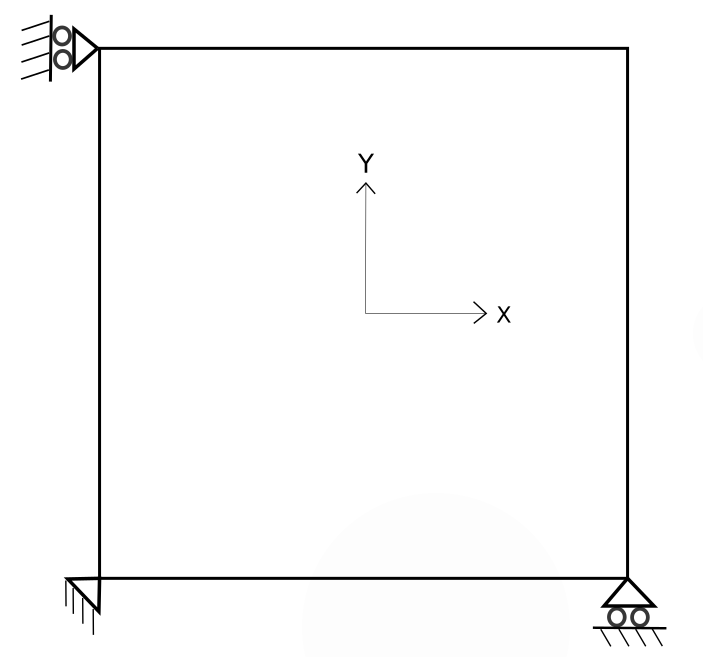
\includegraphics[width=0.8\linewidth]{2DPlate.png}
		\captionof{figure}{2D Plate}
		\label{2Dplate}
	\end{minipage}%
	\begin{minipage}{.4\textwidth}
		\centering
		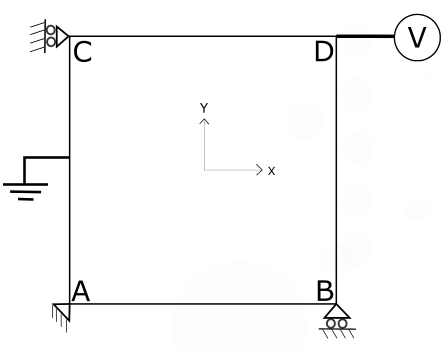
\includegraphics[width=1\linewidth]{PureElectrical.png}
		\captionof{figure}{2D Plate with pure electrical loading}
		\label{PureElectrical22}
	\end{minipage}
\end{figure}
\subsubsection{Parametric details for the plate with single element}


The parametric details for the geometry are the same as in section \hyperref[ParametricDeatils1Elem]{\ref{ParametricDeatils1Elem}}

\subsubsection{Results and discussions}
In this section the comparison is made between IGA code generated result and Abaqus plane strain full integration piezoelectric element (\textbf{CPE4E}) \cite{abaqus10version}.\\The below figures shows the values of Electrical potentials (EPOT) and reactive electrical nodal charge (RCHG) for both Abaqus and IGA element.\\
\\\textbf{*** Electro-mechanical coupling is deactivated in this case by giving all the piezoelectric constants a value of "zero"  }
\\
\textbf{***A similar contour is used for the program generated results and the Abaqus results for easy comparison. }\\
\\
Figure(\ref{E1EPOT}) and Figure(\ref{E1EPOT_IGA}) show the Electrical potential (EPOT) values of the single CPE4E element and single IGA element at 100 \% loading respectively. \\
\begin{figure}[H]
	\centering
	\begin{minipage}{.5\textwidth}
		\centering
		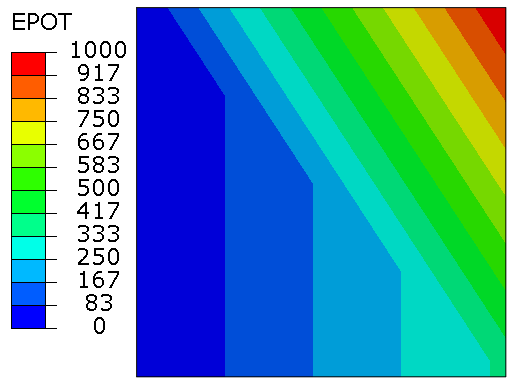
\includegraphics[width=1\linewidth]{E1EPOT.png}
		\captionof{figure}{CPE4E Element:EPOT \\\textbf{Abaqus generated result}}
		\label{E1EPOT}
	\end{minipage}%
	\begin{minipage}{.5\textwidth}
		\centering
		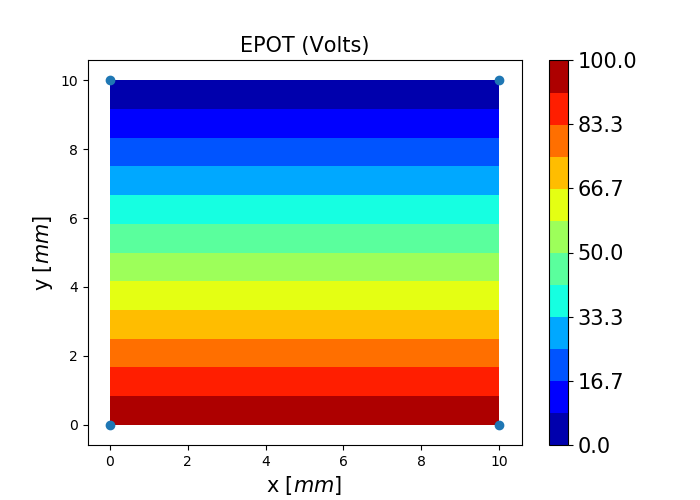
\includegraphics[width=1\linewidth]{E1EPOT_IGA.png}
		\captionof{figure}{IGA Element:EPOT \\ \textbf{Program generated result}}
		\label{E1EPOT_IGA}
	\end{minipage}
\end{figure}
\begin{comment}
\begin{figure}[H]
\begin{center}
\includegraphics[scale=0.45]{xyz.png} 
\caption{\\CPE4 Element U1}\label{xyz}
\end{center}	
\end{figure}

\begin{figure}[H]
\begin{center}
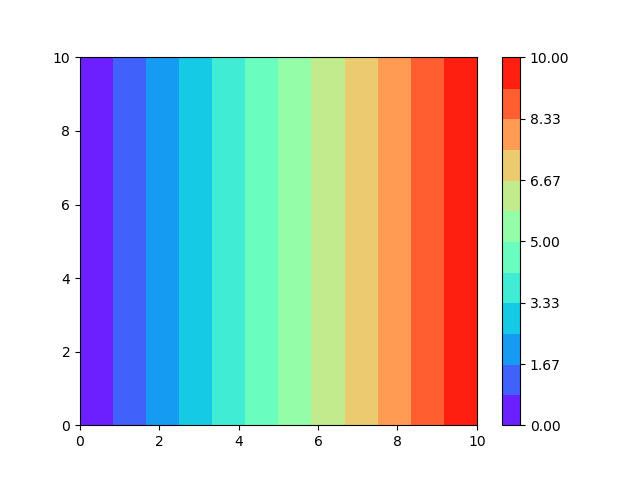
\includegraphics[scale=0.8]{Figure_1.png} 
\caption{\\IGA Element U1}\label{Figure_1}
\end{center}	
\end{figure}
\end{comment}
Figure(\ref{E1RCHG}) and Figure(\ref{E1RCHG_IGA}) show the reactive nodal charge (RCHG) values of the single CPE4E element and single IGA element at 100 \% loading respectively. \\
\begin{figure}[H]
	\centering
	\begin{minipage}{.5\textwidth}
		\centering
		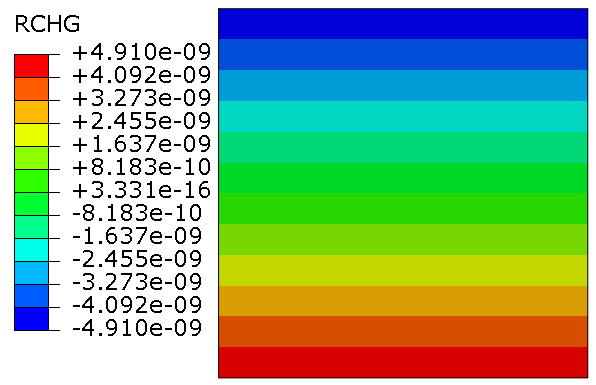
\includegraphics[width=1\linewidth]{E1RCHG.png}
		\captionof{figure}{CPE4 Element:RCHG
		\\\textbf{Abaqus generated result}}
		\label{E1RCHG}
	\end{minipage}%
	\begin{minipage}{.5\textwidth}
		\centering
		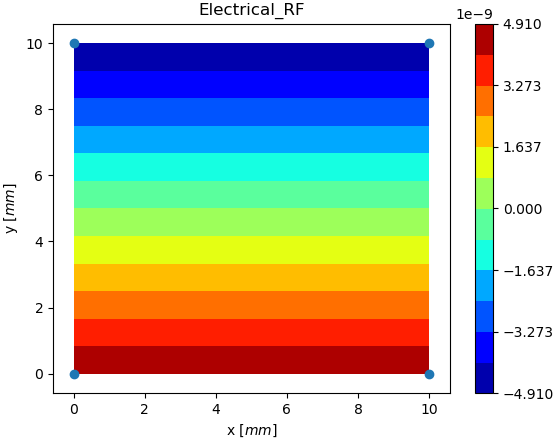
\includegraphics[width=1\linewidth]{E1RCHG_IGA.png}
		\captionof{figure}{IGA Element:RCHG \\ \textbf{Program generated result}}
		\label{E1RCHG_IGA}
	\end{minipage}
\end{figure}

\subsubsection{Conclusion}
As shown in the figures above, the values generated by the IGA code are in line with the results of the Abaqus element. So it can be concluded that for electrical analysis, IGA code written works well with 2D one element case.



\subsection{2D Piezoelectric plate with mechanical loading}
\subsubsection{Problem description} \label{2DPPWMLPD}
A 2D piezoelectric plate subjected to mechanical displacements is considered, as shown in Fig. (\ref{EMLoading}) . The material used is PZT-PIC151 ceramics, and the properties can be seen in the Appendix (\ref{MaterialProps})

\begin{figure}[H]
	\centering
	\begin{minipage}{.5\textwidth}
		\centering
		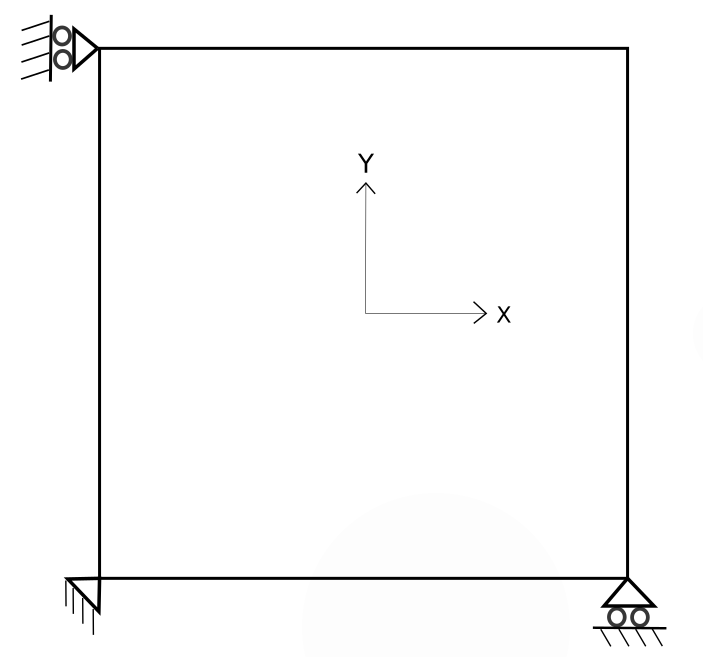
\includegraphics[width=0.8\linewidth]{2DPlate.png}
		\captionof{figure}{2D Piezoelectric Plate}
		\label{2Dplate}
	\end{minipage}%
	\begin{minipage}{.5\textwidth}
		\centering
		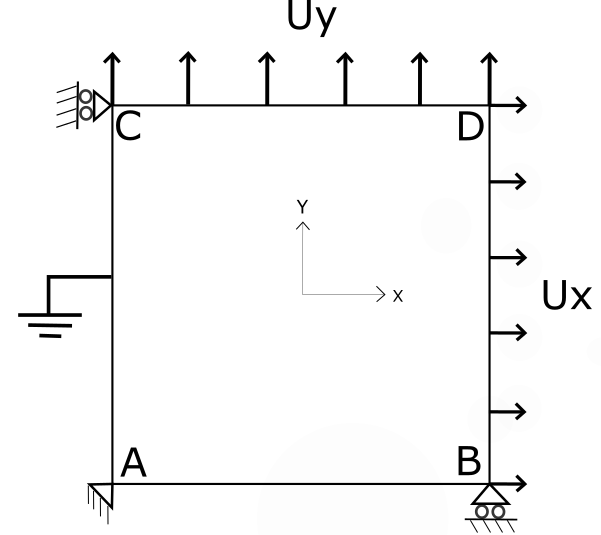
\includegraphics[width=1\linewidth]{Grounded.png}
		\captionof{figure}{2D Piezoelectric Plate with loading}
		\label{EMLoading}
	\end{minipage}
\end{figure}
The movement of the bottom edge AB and left edge AC of 2D piezoelectric plate is fixed in y-direction and x-direction respectively, as shown in figure(\ref{EMLoading}).
The top edge CD is grounded (Electric potential $\Phi = 0$), and a displacement load of 0.1 mm is applied on the right edge BD. The results for a single element case and multiple elements are discussed in the below
sections. \\
The results generated by IGA code is compared with inbuilt Abaqus piezoelectric
element \textbf{CPE4E}.

\subsubsection{Parametric details for the plate with single element}


The parametric details for the geometry are the same as in section \hyperref[ParametricDeatils1Elem]{\ref{ParametricDeatils1Elem}}

\subsubsection{Results and discussions}
Abaqus plane strain full integration piezoelectric element (\textbf{CPE4E}) is used for analysis. The below figures show the values of displacements (U), electrical potentials (EPOT) and the reaction forces (RF ) for both Abaqus and IGA element.\\

Figure(\ref{EM1U1}) and Figure(\ref{EM1U1_IGA}) show the displacement (U1) values of the single CPE4E element and single IGA element at 100 \% loading in x-direction respectively. \\
\begin{figure}[H]
	\centering
	\begin{minipage}{.5\textwidth}
		\centering
		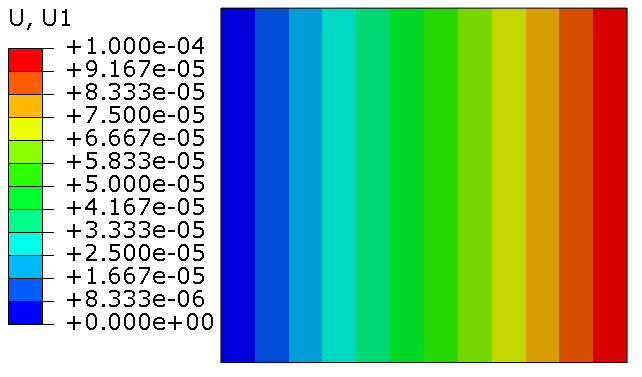
\includegraphics[width=1\linewidth]{EM1U1.png}
		\captionof{figure}{CPE4E Element:U1
		\\\textbf{Abaqus generated result}}
		\label{EM1U1}
	\end{minipage}%
	\begin{minipage}{.5\textwidth}
		\centering
		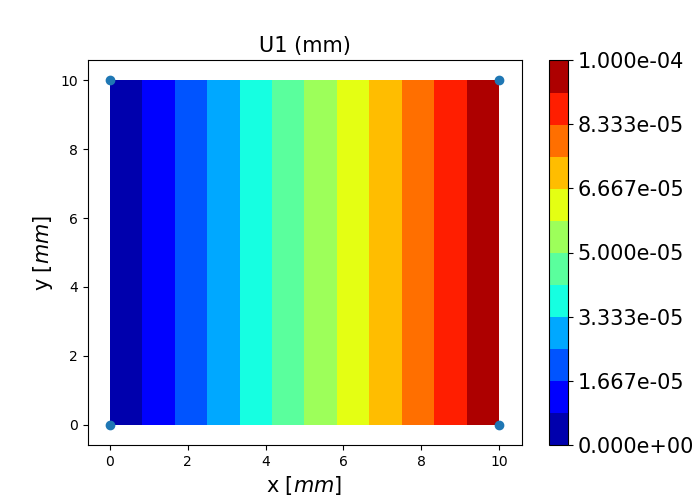
\includegraphics[width=1\linewidth]{EM1U1_IGA.png}
		\captionof{figure}{IGA Piezoelectric Element:U1\\ \textbf{Program generated result}}
		\label{EM1U1_IGA}
	\end{minipage}
\end{figure}
\noindent
Figure(\ref{EM1U2}) and Figure(\ref{EM1U2_IGA}) show the displacement (U2) values of the single CPE4E element and single IGA element at 100 \% loading in y-direction respectively. \\
\begin{figure}[H]
	\centering
	\begin{minipage}{.5\textwidth}
		\centering
		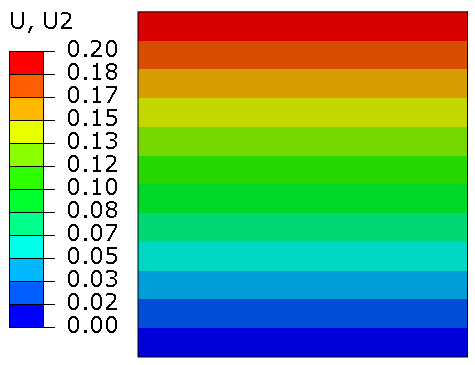
\includegraphics[width=1\linewidth]{EM1U2.png}
		\captionof{figure}{CPE4E Element:U2
		\\\textbf{Abaqus generated result}}
		\label{EM1U2}
	\end{minipage}%
	\begin{minipage}{.5\textwidth}
		\centering
		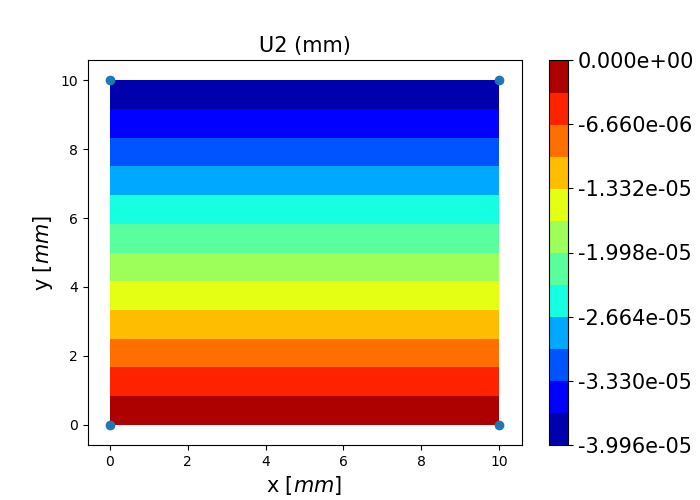
\includegraphics[width=1\linewidth]{EM1U2_IGA.png}
		\captionof{figure}{IGA Piezoelectric Element:U2\\ \textbf{Program generated result}}
		\label{EM1U2_IGA}
	\end{minipage}
\end{figure}
	\begin{comment}
\begin{figure}[H]
	\begin{center}
		\includegraphics[scale=0.45]{xyz.png} 
		\caption{\\CPE4 Element U1}\label{xyz}
	\end{center}	
\end{figure}

\begin{figure}[H]
	\begin{center}
		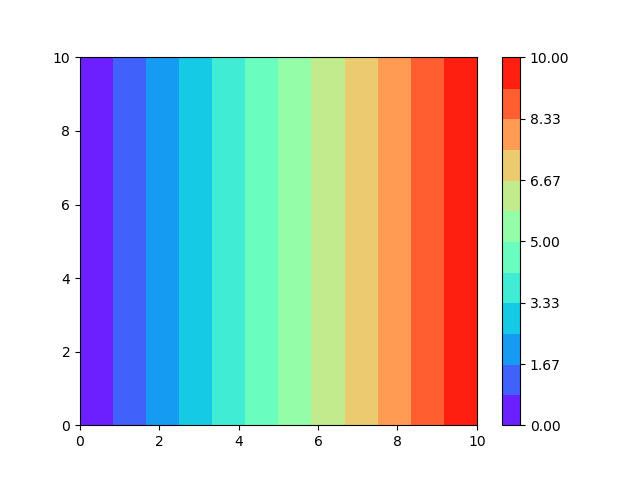
\includegraphics[scale=0.8]{Figure_1.png} 
		\caption{\\IGA Element U1}\label{Figure_1}
	\end{center}	
\end{figure}
	\end{comment}
	


Figure(\ref{EM1RF1}) and Figure(\ref{EM1RF1_IGA}) show the Reaction force values (RF1) of the single CPE4E element and single IGA element at 100 \% loading in x-direction respectively. \\
\begin{figure}[H]
	\centering
	\begin{minipage}{.5\textwidth}
		\centering
		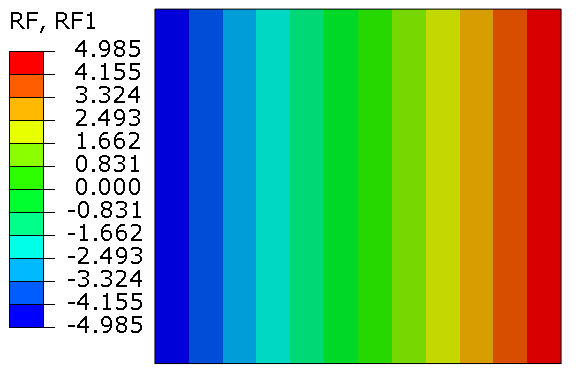
\includegraphics[width=1\linewidth]{EM1RF1.png}
		\captionof{figure}{CPE4E Element:RF1
		\\\textbf{Abaqus generated result}}
		\label{EM1RF1}
	\end{minipage}%
	\begin{minipage}{.5\textwidth}
		\centering
		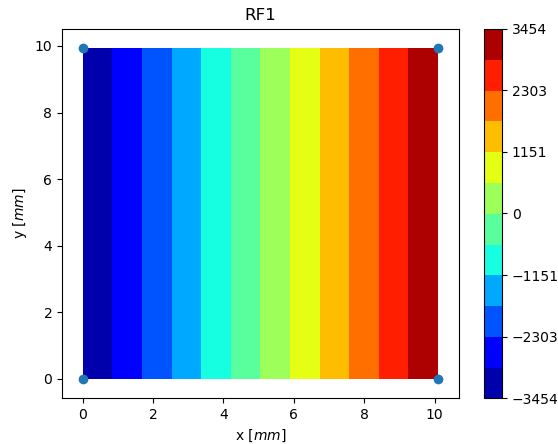
\includegraphics[width=1\linewidth]{EM1RF1_IGA.png}
		\captionof{figure}{IGA Piezoelectric Element:RF1\\ \textbf{Program generated result}}
		\label{EM1RF1_IGA}
	\end{minipage}
\end{figure}



Figure(\ref{EM1EPOT}) and Figure(\ref{EM1EPOT_IGA}) show the Electrical potential values (EPOT) of the single CPE4E element and single IGA element at 100 \% loading respectively. \\
\begin{figure}[H]
	\centering
	\begin{minipage}{.5\textwidth}
		\centering
		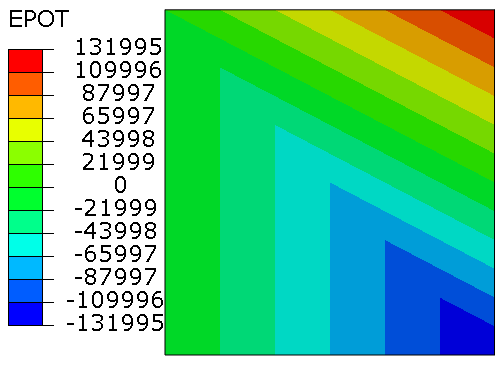
\includegraphics[width=1\linewidth]{EM1EPOT.png}
		\captionof{figure}{CPE4E Element:EPOT
		\\\textbf{Abaqus generated result}}
		\label{EM1EPOT}
	\end{minipage}%
	\begin{minipage}{.5\textwidth}
		\centering
		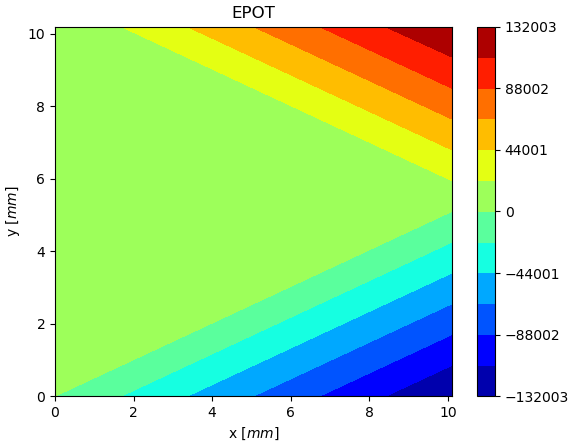
\includegraphics[width=1\linewidth]{EM1EPOT_IGA.png}
		\captionof{figure}{IGA Piezoelectric Element:EPOT\\ \textbf{Program generated result}}
		\label{EM1EPOT_IGA}
	\end{minipage}
\end{figure}
\subsubsection{Conclusion}
As shown in the figures above, the values generated by the IGA code for an electro-mechanical coupling with mechanical input are in line with the results of the Abaqus element. So it can be concluded that IGA code written works well with a 2D one element piezoelectric case with displacement loading.

\subsubsection{Comparison of electro-mechanical coupling with pure mechanical case}
If we consider the problems in section (\ref{2DPWLELPD}) and section (\ref{2DPPWMLPD}), both have same boundary conditions and are loaded in the same way with 0.1 mm displacement in the x-direction. But in the latter case electro-mechanical coupling is taken into consideration.

As seen in the Fig. (\ref{M1RF1_IGA}) and Fig. (\ref{EM1RF1_IGA}) a small difference in reaction force values can be observed due to the considered electro-mechanical coupling in the latter case. Similarly we can find the difference in U2 values as well due to the coupling (refer Fig.(\ref{M1U2_IGA}) and refer Fig. (\ref{EM1U2_IGA}))

\subsubsection{Parametric details for the plate with 2 elements in x-direction and  3 elements in y-direction} \label{ParaMultiEle}
The 2nd order NURBS curve is used in both $\xi$ and $\eta$ directions. \\
\begin{comment}
The knot vectors along $\xi$ and $\eta$ directions are \\
$\Xi= [0,0,1,1]$ and $\eta= [0,0,1,1]$. \\
Control points along $\xi$ direction is given by \\
$n_{cp}(\xi)$ = total number of knots in $[\Xi] - (p+1) = 2$.\\
Similarly the total number of control points along $\eta$ direction is given
by\\ $n_{cp}(\eta)$ = total number of knots in $[H ]- (q+1) = 2$ . \\
The total number of control points which defines the surface is\\
$n_{cp}$ = $n_{cp}(\xi) * n_{cp}(\eta)$ which is $2*2 = 4$. \\
\end{comment}
\begin{comment}
\item Control points net for the geometry \\
P = [[[0,0,0,1],[L,0,0,1]],
[[0,L,0,1],[L,L,0,1]]]

$$
P = \begin{bmatrix}
[0,0,0,1] & [L,0,0,1] \\
[L,0,0,1] & [L,L,0,1] \\
\end{bmatrix} 
$$

\end{enumerate}
%\end{verbatim}
\end{comment}
%\begin{verbatim}
\begin{enumerate}
	\item Physical details for the geometry: \\
	L = 10 \qquad \# Length of the plate in mm \\
	H = 10 \qquad \# Height of the plate in mm \\
	T = 1 {} \qquad \# Thickness of the plate in mm \\
	
	\item Parametric details of the geometry: \\
	$\Xi$ =  [0,0,1,2,2] \qquad \# Knot vector in xi  direction \\
	$H$ = [0,0,1,2,3,3] \qquad \# Knot vector in eta direction \\
	
	Degree of the curve \\
	p=1 \qquad \# Degree of the curve in $\xi$  direction \\
	q=1 \qquad \# Degree of the curve in $\eta$ direction \\
	
	Number of control points in each direction \\
	$n_{cp}^{\xi}$  = len($\Xi$) - (p+1)  \qquad \#No.of control points in $\xi$
	direction (5-(1+1) = 3) \\
	$n_{cp}^{\eta}$ = len($H$) - (q+1)  \qquad \#No.of control points in $\eta$
	direction (6-(1+1) = 4) \\
	
	\item Total number of control points for the geometry \\
	$n_{cp} = n_{cp}^{\xi} * n_{cp}^{\eta}$ = 3*4 = 12\\
	The control points are given by
	\begin{center}
		\begin{tabular}{ |c|c|c|c|c|c| } 
			\hline
			i & $ P_{i,0} $ & $ P_{i,1} $ & $ P_{i,2} $   \\ \hline
			0 & $ (0,0,0,1) $ & $ (0,5,0,1) $ & $ (0,10,0,1) $  \\ \hline
			1 & $ (3.33,0,0,1) $ & $ (3.33,5,0,1) $ & $ (3.33,10,0,1) $  \\ \hline
			2 & $ (6.67,0,0,1) $ & $ (6.67,5,0,1) $ & $ (6.67,10,0,1) $  \\ \hline
			3 & $ (10,0,0,1) $ & $ (10,5,0,1) $ & $ (10,10,0,1) $  \\ \hline
		\end{tabular}
	\end{center}
	with fourth value in the parentheses being weights of respective control points.
	A control point assembly array and knot vector connectivity matrix are used to connect the elements.
\end{enumerate}

\subsubsection{Results and discussions}
Abaqus plane strain full integration piezoelectric element (\textbf{CPE4E}) is used for analysis. For the comparison between Abaqus and IGA elements, 2 elements, along the x-direction and 3 elements along the y-direction, are used. A different number of elements are used along each direction in order to verify if the code generates proper results in unsymmetric conditions as well w.r.t number of elements in each direction.\\
The \textbf{blue points} on the program generated results are the final position of the control points at 100 \% loading.\\
The below figures shows the values of displacements (U), electrical potentials (EPOT) and reaction forces (RF ) for both Abaqus and IGA elements.\\
Figure(\ref{EM23U1}) and Figure(\ref{EM23U1_IGA}) show the displacement (U1) values of the CPE4E elements and IGA elements at 100 \% loading in x-direction respectively. \\
\begin{figure}[H]
	\centering
	\begin{minipage}{.5\textwidth}
		\centering
		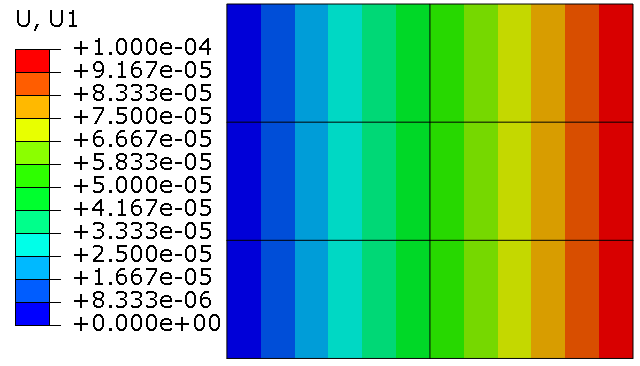
\includegraphics[width=1\linewidth]{EM23U1.png}
		\captionof{figure}{CPE4E Element:U1
		\\\textbf{Abaqus generated result}}
		\label{EM23U1}
	\end{minipage}%
	\begin{minipage}{.5\textwidth}
		\centering
		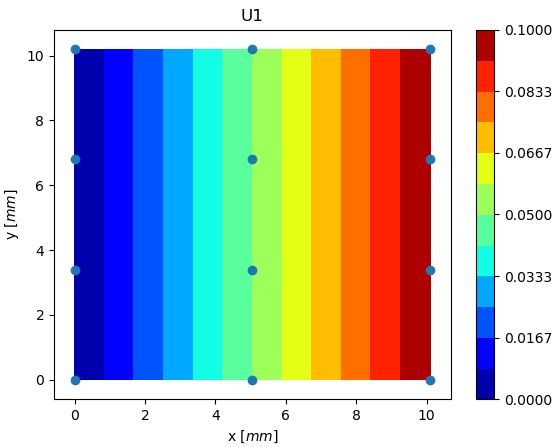
\includegraphics[width=1\linewidth]{EM23U1_IGA.png}
		\captionof{figure}{IGA Piezoelectric Element:U1\\ \textbf{Program generated result}}
		\label{EM23U1_IGA}
	\end{minipage}
\end{figure}
\noindent
Figure(\ref{EM23U2}) and Figure(\ref{EM23U2_IGA}) show the displacement (U2) values of the CPE4E elements and the IGA elements at 100 \% loading in the y-direction respectively. \\
\begin{comment}
\begin{figure}[H]
\begin{center}
\includegraphics[scale=0.45]{xyz.png} 
\caption{\\CPE4 Element U1}\label{xyz}
\end{center}	
\end{figure}

\begin{figure}[H]
\begin{center}
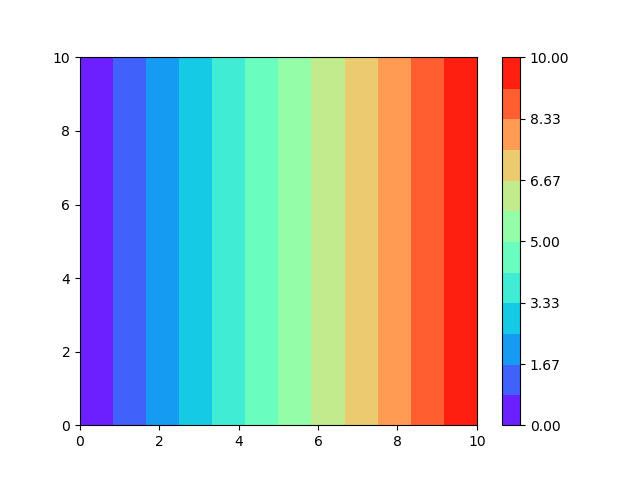
\includegraphics[scale=0.8]{Figure_1.png} 
\caption{\\IGA Element U1}\label{Figure_1}
\end{center}	
\end{figure}
\end{comment}
\begin{figure}[H]
	\centering
	\begin{minipage}{.5\textwidth}
		\centering
		\includegraphics[width=1\linewidth]{EM23U2.png}
		\captionof{figure}{CPE4E Element:U2
		\\\textbf{Abaqus generated result}}
		\label{EM23U2}
	\end{minipage}%
	\begin{minipage}{.5\textwidth}
		\centering
		\includegraphics[width=1\linewidth]{EM23U2_IGA.png}
		\captionof{figure}{IGA Piezoelectric Element:U2\\ \textbf{Program generated result}}
		\label{EM23U2_IGA}
	\end{minipage}
\end{figure}
Figure(\ref{EM23RF1}) and Figure(\ref{EM23RF1_IGA}) show the Reaction force values (RF1) of the CPE4E elements and the IGA elements at 100 \% loading in x-direction respectively. \\
\begin{figure}[H]
	\centering
	\begin{minipage}{.5\textwidth}
		\centering
		\includegraphics[width=1\linewidth]{EM23RF1.png}
		\captionof{figure}{CPE4E Element:RF1
		\\\textbf{Abaqus generated result}}
		\label{EM23RF1}
	\end{minipage}%
	\begin{minipage}{.5\textwidth}
		\centering
		\includegraphics[width=1\linewidth]{EM23RF1_IGA.png}
		\captionof{figure}{IGA Piezoelectric Element:RF1\\ \textbf{Program generated result}}
		\label{EM23RF1_IGA}
	\end{minipage}
\end{figure}

Figure(\ref{EM23EPOT}) and Figure(\ref{EM23EPOT_IGA}) show the Electrical potential values (EPOT) of the CPE4E elements and the IGA elements at 100 \% loading respectively. \\
\begin{figure}[H]
	\centering
	\begin{minipage}{.5\textwidth}
		\centering
		\includegraphics[width=1\linewidth]{EM23EPOT.png}
		\captionof{figure}{CPE4E Element:EPOT
		\\\textbf{Abaqus generated result}}
		\label{EM23EPOT}
	\end{minipage}%
	\begin{minipage}{.5\textwidth}
		\centering
		\includegraphics[width=1\linewidth]{EM23EPOT_IGA.png}
		\captionof{figure}{IGA Piezoelectric Element:EPOT\\ \textbf{Program generated result}}
		\label{EM23EPOT_IGA}
	\end{minipage}
\end{figure}

\subsubsection{Conclusion}
As shown in figures above for a 6 elements case, the results generated by IGA code are in line with the results of the Abaqus elements.  





\subsection{2D Piezoelectric plate with electrical loading}
\subsubsection{Problem description} \label{2DPPWEL}
A 2D piezoelectric plate subjected to electrical loading is considered, as shown in Fig. (\ref{PureElectrical}) . The material used is PZT-PIC151 ceramics, and the properties can be seen in the Appendix (\ref{MaterialProps})

\begin{figure}[H]
	\centering
	\begin{minipage}{.5\textwidth}
		\centering
		\includegraphics[width=0.8\linewidth]{2DPlate.png}
		\captionof{figure}{2D Piezoelectric Plate}
		\label{2Dplate}
	\end{minipage}%
	\begin{minipage}{.4\textwidth}
		\centering
		\includegraphics[width=1\linewidth]{PureElectrical.png}
		\captionof{figure}{2D Piezoelectric Plate with loading}
		\label{PureElectrical}
	\end{minipage}
\end{figure}
The movement of the bottom edge AB and left edge AC of 2D piezoelectric plate is fixed in y-direction and x-direction respectively, as shown in figure(\ref{PureElectrical}).
The top edge CD is grounded (Electric potential $\Phi = 0$), and an electrical potential of 1000 V  is applied on the bottom edge AB. The results for a single element case and multiple elements are discussed in the below
sections. \\
The results generated by IGA code is compared with inbuilt Abaqus piezoelectric
element \textbf{CPE4E}.

\subsubsection{Parametric details for the plate with single element}


The parametric details for the geometry are the same as in section \hyperref[ParametricDeatils1Elem]{\ref{ParametricDeatils1Elem}}

\subsubsection{Results and discussions}
Abaqus plane strain full integration piezoelectric element (\textbf{CPE4E}) is used for analysis. The below figures show the values of displacements (U), electrical potentials (EPOT) and the reactive electrical nodal charge (RCHG) for both Abaqus and IGA element.\\

Figure(\ref{EME1U1}) and Figure(\ref{EME1U1_IGA}) show the displacement (U1) values of the single CPE4E element and single IGA element at 100 \% loading in x-direction respectively. \\
\begin{figure}[H]
	\centering
	\begin{minipage}{.5\textwidth}
		\centering
		\includegraphics[width=1\linewidth]{EME1U1.png}
		\captionof{figure}{CPE4E Element:U1
			\\\textbf{Abaqus generated result}}
		\label{EME1U1}
	\end{minipage}%
	\begin{minipage}{.5\textwidth}
		\centering
		\includegraphics[width=1\linewidth]{EME1U1_IGA.png}
		\captionof{figure}{IGA Piezoelectric Element:U1\\ \textbf{Program generated result}}
		\label{EME1U1_IGA}
	\end{minipage}
\end{figure}
\noindent
Figure(\ref{EME1U2}) and Figure(\ref{EME1U2_IGA}) show the displacement (U2) values of the single CPE4E element and single IGA element at 100 \% loading in y-direction respectively. \\
\begin{figure}[H]
	\centering
	\begin{minipage}{.5\textwidth}
		\centering
		\includegraphics[width=1\linewidth]{EME1U2.png}
		\captionof{figure}{CPE4E Element:U2
			\\\textbf{Abaqus generated result}}
		\label{EME1U2}
	\end{minipage}%
	\begin{minipage}{.5\textwidth}
		\centering
		\includegraphics[width=1\linewidth]{EME1U2_IGA.png}
		\captionof{figure}{IGA Piezoelectric Element:U2\\ \textbf{Program generated result}}
		\label{EME1U2_IGA}
	\end{minipage}
\end{figure}
\begin{comment}
\begin{figure}[H]
\begin{center}
\includegraphics[scale=0.45]{xyz.png} 
\caption{\\CPE4 Element U1}\label{xyz}
\end{center}	
\end{figure}

\begin{figure}[H]
\begin{center}
\includegraphics[scale=0.8]{Figure_1.png} 
\caption{\\IGA Element U1}\label{Figure_1}
\end{center}	
\end{figure}
\end{comment}


Figure(\ref{EME1EPOT}) and Figure(\ref{EME1EPOT_IGA}) show the Electrical potential values (EPOT) of the single CPE4E element and single IGA element at 100 \% loading respectively. \\
\begin{figure}[H]
	\centering
	\begin{minipage}{.5\textwidth}
		\centering
		\includegraphics[width=1\linewidth]{EME1EPOT.png}
		\captionof{figure}{CPE4E Element:EPOT
			\\\textbf{Abaqus generated result}}
		\label{EME1EPOT}
	\end{minipage}%
	\begin{minipage}{.5\textwidth}
		\centering
		\includegraphics[width=1\linewidth]{EME1EPOT_IGA.png}
		\captionof{figure}{IGA Piezoelectric Element:EPOT\\ \textbf{Program generated result}}
		\label{EME1EPOT_IGA}
	\end{minipage}
\end{figure}

Figure(\ref{EME1RCHG}) and Figure(\ref{EME1RCHG_IGA}) show the Reactive electrical nodal charge (RCHG) of the single CPE4E element and single IGA element at 100 \% loading respectively. \\
\begin{figure}[H]
	\centering
	\begin{minipage}{.5\textwidth}
		\centering
		\includegraphics[width=1\linewidth]{EME1RCHG.png}
		\captionof{figure}{CPE4E Element:RCHG
			\\\textbf{Abaqus generated result}}
		\label{EME1RCHG}
	\end{minipage}%
	\begin{minipage}{.5\textwidth}
		\centering
		\includegraphics[width=1\linewidth]{EME1RCHG_IGA.png}
		\captionof{figure}{IGA Piezoelectric Element:RCHG\\ \textbf{Program generated result}}
		\label{EME1RCHG_IGA}
	\end{minipage}
\end{figure}
\subsubsection{Conclusion}
As shown in the figures above, the values generated by the IGA code for an electro-mechanical coupling with electrical input are in line with the results of the Abaqus element. So it can be concluded that IGA code written works well with a 2D one element piezoelectric case with a given voltage difference on the surface.

\subsubsection{Comparison of electro-mechanical coupling with pure electrical case}
Considering the problems in section (\ref{2DPWPELPD}) and section (\ref{2DPPWEL}), the 2D plate is grounded on the top edge and applied a potential of 1000 V on the bottom edge. But in the latter case electro-mechanical coupling is taken into consideration.
As seen in the Fig. (\ref{E1RCHG_IGA}) and Fig. (\ref{EME1RCHG_IGA}) a small difference in RCHG values can be observed due to the considered electro-mechanical coupling in the latter case.

\subsubsection{Parametric details for the plate with 2 elements in x-direction and  3 elements in y-direction}

The parametric details for the geometry are the same as in section \hyperref[ParaMultiEle]{\ref{ParaMultiEle}}

\subsubsection{Results and discussions}
Abaqus plane strain full integration piezoelectric element (\textbf{CPE4E}) is used for analysis. For the comparison between Abaqus and IGA elements, 2 elements, along the x-direction and 3 elements along the y-direction, are used.\\
The below figures shows the values of displacements (U), electrical potentials (EPOT) and reactive electrical nodal charge (RCHG) for both Abaqus and IGA elements.\\
Figure(\ref{EME23U1}) and Figure(\ref{EME23U1_IGA}) show the displacement (U1) values of the CPE4E elements and IGA elements at 100 \% loading in x-direction respectively. \\
\begin{figure}[H]
	\centering
	\begin{minipage}{.5\textwidth}
		\centering
		\includegraphics[width=1\linewidth]{EME23U1.png}
		\captionof{figure}{CPE4E Element:U1
			\\\textbf{Abaqus generated result}}
		\label{EME23U1}
	\end{minipage}%
	\begin{minipage}{.5\textwidth}
		\centering
		\includegraphics[width=1\linewidth]{EME23U1_IGA.png}
		\captionof{figure}{IGA Piezoelectric Element:U1\\ \textbf{Program generated result}}
		\label{EME23U1_IGA}
	\end{minipage}
\end{figure}
\noindent
Figure(\ref{EME23U2}) and Figure(\ref{EME23U2_IGA}) show the displacement (U2) values of the CPE4E elements and the IGA elements at 100 \% loading in the y-direction respectively. \\
\begin{comment}
\begin{figure}[H]
\begin{center}
\includegraphics[scale=0.45]{xyz.png} 
\caption{\\CPE4 Element U1}\label{xyz}
\end{center}	
\end{figure}

\begin{figure}[H]
\begin{center}
\includegraphics[scale=0.8]{Figure_1.png} 
\caption{\\IGA Element U1}\label{Figure_1}
\end{center}	
\end{figure}
\end{comment}
\begin{figure}[H]
	\centering
	\begin{minipage}{.5\textwidth}
		\centering
		\includegraphics[width=1\linewidth]{EME23U2.png}
		\captionof{figure}{CPE4E Element:U2
			\\\textbf{Abaqus generated result}}
		\label{EME23U2}
	\end{minipage}%
	\begin{minipage}{.5\textwidth}
		\centering
		\includegraphics[width=1\linewidth]{EME23U2_IGA.png}
		\captionof{figure}{IGA Piezoelectric Element:U2\\ \textbf{Program generated result}}
		\label{EME23U2_IGA}
	\end{minipage}
\end{figure}

Figure(\ref{EME23EPOT}) and Figure(\ref{EME23EPOT_IGA}) show the Electrical potential values (EPOT) of the CPE4E elements and the IGA elements at 100 \% loading respectively. \\
\begin{figure}[H]
	\centering
	\begin{minipage}{.5\textwidth}
		\centering
		\includegraphics[width=1\linewidth]{EME23EPOT.png}
		\captionof{figure}{CPE4E Element:EPOT
			\\\textbf{Abaqus generated result}}
		\label{EME23EPOT}
	\end{minipage}%
	\begin{minipage}{.5\textwidth}
		\centering
		\includegraphics[width=1\linewidth]{EME23EPOT_IGA.png}
		\captionof{figure}{IGA Piezoelectric Element:EPOT\\ \textbf{Program generated result}}
		\label{EME23EPOT_IGA}
	\end{minipage}
\end{figure}

Figure(\ref{EME23RCHG}) and Figure(\ref{EME23RCHG_IGA}) show the Reactive electrical nodal charge (RCHG) of the CPE4E elements and IGA elements at 100 \% loading respectively. \\
\begin{figure}[H]
	\centering
	\begin{minipage}{.5\textwidth}
		\centering
		\includegraphics[width=1\linewidth]{EME23RCHG.png}
		\captionof{figure}{CPE4E Element:RCHG
			\\\textbf{Abaqus generated result}}
		\label{EME23RCHG}
	\end{minipage}%
	\begin{minipage}{.5\textwidth}
		\centering
		\includegraphics[width=1\linewidth]{EME23RCHG_IGA.png}
		\captionof{figure}{IGA Piezoelectric Element:RCHG\\ \textbf{Program generated result}}
		\label{EME23RCHG_IGA}
	\end{minipage}
\end{figure}

\subsubsection{Conclusion}
As shown in figures above for a 6 elements case, the results generated by IGA code are in line with the results of the Abaqus elements.  




 



\newpage
\section{Milestones achieved}
The following table describes the proposed coding activities and achieved activities.
\begin{center}
	\begin{tabular}{ |c|c|c|c| } 
		\hline
		Proposed Activities & Achieved \\
		\hline 
		NURBS based 2D geometry generation & yes \\
		Implementation of the Isogeometric Analysis for a single element 2D case & yes \\  
		Coupling between mechanical and electrical Dof’s & yes \\ 
		Verification of results with abaqus inbuilt piezoelectric element & \\
		for mechanical input and electro-mecanical output & yes \\ 
		Verification of results with abaqus inbuilt piezoelectric element & \\
		for electrical input and electro-mecanical output & yes \\ 
		\hline
		Extra Activities & Achieved \\
		\hline
		Code extension to do analysis with multiple elements & yes \\
		Implementation of Knot and Control point assembly arrays & yes \\
		\hline
	\end{tabular}
\end{center}

\section{Intricacies of Isogeometric analysis}
To develop a code for Isogeometric analysis, it demands the understanding of NURBS theory, apart from the knowledge in the field of FEM. Although the NURBS book gives a clear picture of how to generate a curve and a surface, it is not designed to give a clear insight on how to work with Isogeometric analysis. For example, we can find the derivatives of the NURBS basis functions only but not the derivatives of bivariate basis functions (which are used in NURBS surface). Since basis functions are of recursive nature, it is no more straight forward to derivate the functions and requires a deep insight into the theory that goes with it. One can find much material regarding IGA analysis online, but when it comes to derivatives of bivariate basis functions, there is not much to refer. It took time and effort to get the right combination of material to understand the way to derivate, and the next major task is to write code. As the NURBS basis functions are defined in parametric space, as discussed in section(\ref{ProcessingStage}), it is not straight forward to map physical space on to master space like in FEM. The addition of parametric space makes things a little complicated because the derivatives have to be defined in three different spaces. An introduction paper on IGA by Vishal et al. \cite{agrawal2019iga} , gave a clear picture of these mappings. Unlike FEM, which contains a fixed number of nodes, this is not the case with IGA, where the number of control points (equivalent term to nodes in FEM) in each element depends on the parametric details of the NURBS curve/surface. A generalized way has to be adopted to formulate matrices involved in the analysis (like B matrix, Stiffness matrix, DOF array and Global force array) so that it does not require to reformulate the code every time the parametric details change (which is the primary purpose of IGA to reduce the time involved in meshing the geometry as in FEM). Moreover, extending a code from a single element to multiple elements requires two types of connecting arrays namely knot and control points connectivity arrays as discussed in section(\ref{AssemblyArrays}). So the code has to handle additional connectivity. Lastly defining boundary conditions need special techniques, unlike FEM.

\newpage
\section{Conclusion}
In this project, an Isogeometric analysis code is developed to create NURBS surface using parametric details and use the same basis functions to analyze Linear elastic mechanical loading and later extended to electro-mechanical coupling. The code is written in such a way that, it can analyze a 2D geometry with up to 4th order NURBS basis functions ( the order of the basis functions in each direction can vary, for example, a surface can be generated using 3rd order basis functions in $\xi$ direction and 2nd order basis functions in $\eta$ direction). The drawback of the written code is, it gives accurate results for a 2nd order NURBS basis functions but fails to produce correct results for higher-order basis functions. This is because unlike FEM, where boundary conditions can be applied on nodes, the same procedure cannot be followed for IGA where basis functions have higher continuity, unlike $C^0$ continuity at nodes in FEM. The results of the IGA code are verified with the Abaqus elements for 2nd order NURBS 	curve.

\subsection{Continuation Strategy}

The existing code can be extended by adding boundary condition defining techniques like least square minimization to identify the boundary controlling points and assigning appropriate boundary conditions. The code can be further extended to 3D geometry, but coding assembly arrays ( knot connectivity and control points assembly arrays ) would be challenging.


\newpage
\section{Appendices}

\subsection{Material Properties} \label{MaterialProps}
The material used is
PZT-PIC151 ceramics and the properties \cite{kozinov2018simulation} are as follow. The elastic constants (C) are transversely isotropic, dielectric constants ($\kappa$) are anisotropic and material is polarized in Y-direction. 

$$
C = \begin{bmatrix}
139000 & 74280 & 77840 & 0 & 0 & 0\\
47280 & 115400 & 74280 & 0 & 0 & 0\\
77840 & 74280 & 139000 & 0 & 0 & 0\\
0 & 0 & 0 & 25640 & 0 & 0\\
0 & 0 & 0 & 0 & 25640 & 0\\
0 & 0 & 0 & 0 & 0 & 25640\\
\end{bmatrix} MPa
$$  
$$
e = \begin{bmatrix}
0 & -5.20710E-6 & 0 \\
0 & 15.08E-6 & 0 \\
0 & -5.207E-6 & 0\\
12.710E-6 & 0 & 0 \\
0 & 0 & 0 \\
0 & 0 & 12.710E-6 \\
\end{bmatrix} C/ mm`2
$$
$$
\varepsilon = \begin{bmatrix}
6.752E-12 & 0 & 0 \\
0 & 5.872E-12 & 0 \\
0 & 0 & 6.752E-12\\
\end{bmatrix} C/(V mm)
$$
where \\
e is Piezoelectric constants.








\noindent
%*** Remember References and citations ***
\bibliographystyle{plain}
\bibliography{References} 
\end{document}